% Escolha: Portugues ou Ingles ou Espanhol.
% Para a versão final do texto, após a defesa, acrescente Final:

\documentclass[Ingles]{ic-tese-v3}
%\documentclass[Portugues,Final]{ic-tese-v3}

\usepackage[latin1,utf8]{inputenc}

% Para acrescentar comentários ao PDF descomente:
\usepackage
%  [pdfauthor={nome do autor},
%   pdftitle={titulo},
%   pdfkeywords={palavra-chave, palavra-chave},
%   pdfproducer={Latex with hyperref},
%   pdfcreator={pdflatex}]
{hyperref}

\usepackage{hyperref}
\usepackage{ae}
\usepackage{indentfirst}
\usepackage{colortbl}
\usepackage{amssymb,amsmath,graphicx,fancyhdr,psfrag,tabularx,float,textcomp,fancybox,amsfonts}
\usepackage{algorithmic}
\usepackage{color}
\usepackage{rotating}
\usepackage{epsfig}
\usepackage{ifthen}
\usepackage{lscape}
\usepackage{array}
\usepackage{forest}
\usepackage{setspace}
\usepackage{xcolor}
\usepackage{lipsum}
\usepackage{pbox}
\usepackage{multirow}
\RequirePackage{multicol}
\usepackage{adjustbox}
\usepackage{caption}
\usepackage{longtable}
\usepackage[autostyle]{csquotes}
\usepackage{comment}
\usepackage{enumerate}
\usepackage{manyfoot}
\usepackage{listings}
\usepackage{arydshln}
\usetikzlibrary{arrows,shapes}
\usepackage{pgf-pie}
\usepackage{bbding}
\usepackage{url}
\usepackage{verbatim}
\usepackage{booktabs}
\usepackage{siunitx}
\usepackage{makecell}
\usepackage{pifont}
\usepackage{natbib}
\usepackage[noabbrev,nameinlink,capitalise]{cleveref}
\usepackage{eqparbox}
\usepackage{enumitem}

% algorithms
\usepackage[english,ruled,lined,linesnumbered]{algorithm2e} % Escrever algoritmos

% images
\usepackage{tikz}
\usepackage{pgf}
\usepackage{pgfplots}
\usepackage{geometry}
\usepackage{subcaption}

% fonts
\usepackage[utf8]{inputenc}
\usepackage[english]{babel}
\usepackage{amsthm}

% math
\usepackage{calc}% http://ctan.org/pkg/calc
\usepackage[T1]{fontenc}
\usepackage{theoremref}

% read data
\usepackage{readarray,tokcycle}

\SetKwInput{Input}{Input}%
\SetKwInput{Output}{Output}%

\newtheorem{property}{Property}
\newtheorem{proposition}{Proposition}
\newtheorem{definition}{Definition}

\newcommand{\z}{$\bullet$}
\newcommand{\drawBlock}[3]{
  \draw [fill=#3, draw = white] (#1) \foreach \v [count=\i] in #2 {
    \ifnum\i>1
      -- (\v)
    \fi
  } -- cycle;
}
\newcommand{\drawArcs}[3]{
  \foreach \i in {1,...,#2}{
    \draw [#3] (#1[\i,1]) -- (#1[\i,2]);
  }
}
\newcommand{\drawArcsBend}[3]{
  \foreach \i in {1,...,#2}{
    \draw [#3] (#1[\i,1]) to [bend right=3] (#1[\i,2]);
  }
}

%%%%%%%%%%%%%%%%%%%%%%%%%%%%%%%%%%%%
%%%%%%%%%% Tikz settings %%%%%%%%%%%
%%%%%%%%%%%%%%%%%%%%%%%%%%%%%%%%%%%%

\usetikzlibrary{arrows.meta,arrows}
\usetikzlibrary{arrows,positioning,automata,shadows,fit,shapes,calc,shapes.geometric}
\usetikzlibrary{decorations.pathmorphing}
\tikzset{triangle_black/.style={regular polygon, regular polygon sides=3, minimum size=0.3cm, fill=black}}
\tikzset{triangle/.style={regular polygon, regular polygon sides=3, minimum size=0.3cm, fill=white}}
\tikzset{square/.style={regular polygon, regular polygon sides=4, minimum size=0.3cm, fill=white}}
\tikzset{circufe/.style={circle,draw, minimum size=0.2cm, fill=white}}
\tikzset{raio/.style={circle,draw, minimum size=1.45cm, fill=white}} 
\tikzset{circle_new/.style={circle,draw, minimum size=0.2cm, fill=white}}   
\geometry{
  a4paper,
%  total={170mm,257mm},
  left=1in,
  top=1in,
  bottom=1in,
  right=1in
}

\usepackage{glossaries}

\makeglossaries
\newacronym{ew}{EW}{Epidemiological Week}
\newacronym{ml}{ML}{Machine Learning}
\newacronym{gis}{GIS}{Geographic Information System}
\newacronym{paho}{PAHO}{Pan American Health Organization}
\newacronym{who}{WHO}{World Health Organization}
\newacronym{or}{OR}{Operations Research}
\newacronym{osm}{OSM}{Open Street Maps}
\newacronym{mabs}{MABS}{Multi-Agent-Based Simulation}
\newacronym{ode}{ODE}{Ordinary Differential Equations}
\newacronym{darp}{Dengue-PARP}{Dengue Prize-collecting Arc Routing Problem}
\newacronym{sinan}{SINAN}{Information System for Notifiable Disease}
\newacronym{ibge}{IBGE}{Brazilian Institute of Geography and Statistics}
\newacronym{mae}{MAE}{Mean Absolute Error}
\newacronym{vrp}{VRP}{Vehicle Routing Problem}
\newacronym{arp}{ARP}{Arc Routing Problem}
\newacronym{cbrp}{CBRP}{City Block Routing Problem}
\newacronym{ilp}{ILP}{Integer Linear Programming}
\newacronym{milp}{MILP}{Mixed Interger Linear Programming}
\newacronym{mtz}{MTZ}{Miller-Tucker-Zemlin}
\newacronym{scbrp}{SCBRP}{Stochastic City Block Routing Problem}
\newacronym{lr}{LR}{Lagrangean Relaxation}
\newacronym{lpp}{LPP}{Lagrangian Primal Problem}
\newacronym{ldp}{LDP}{Lagrangian Dual Problem}



\begin{document}

% Escolha entre autor ou autora:
\autor{Carlos Victor Dantas Araújo}
%\autora{Nome da Autora}

% Sempre deve haver um título em português:
% \titulo{Dengue Control}

% Se a língua for o inglês ou o espanhol defina:
\title{Dengue Control}

% Escolha entre orientador ou orientadora. Inclua os títulos acadêmicos:
\orientador{Prof. Dr. Fábio Luiz Usberti}
%\orientadora{Profa. Dra. Nome da Orientadora}

% Escolha entre coorientador ou coorientadora, se houver.  Inclua os títulos acadêmicos:
%\coorientador{Prof. Dr. Eng. Lic. Nome do Co-Orientador}
%\coorientadora{Profa. Dra. Eng. Lic. Nome da Co-Orientadora}

% Escolha entre mestrado ou doutorado:
% \mestrado
\doutorado

% Se houve cotutela, defina:
%\cotutela{Universidade Nova de Plutão}

\datadadefesa{22}{09}{2025}

% Para a versão final defina:
%\avaliadorA{Prof. Dr. Primeiro Avaliador}{Instituição do primeiro avaliador}
%\avaliadorB{Profa. Dra. Segunda Avaliadora}{Instituição da segunda avaliadora}
%\avaliadorC{Dr. Terceiro Avaliador}{Instituição do terceiro avaliador}
%\avaliadorD{Prof. Dr. Quarto Avaliador}{Instituição do quarto avaliador}
%\avaliadorE{Prof. Dr. Quinto Avaliador}{Instituição do quinto avaliador}
%\avaliadorF{Prof. Dr. Sexto Avaliador}{Instituição do sexto avaliador}
%\avaliadorG{Prof. Dr. Sétimo Avaliador}{Instituição do sétimo avaliador}
%\avaliadorH{Prof. Dr. Oitavo Avaliador}{Instituição do oitavo avaliador}


% Para incluir a ficha catalográfica em PDF na versão final, descomente e ajuste:
%\fichacatalografica{arquivo.pdf}


% Este comando deve ficar aqui:
\paginasiniciais


% Se houver dedicatória, descomente:
%\prefacesection{Dedicatória}
%A dedicatória deve ocupar uma única página.


% Se houver epígrafe, descomente e edite:
% \begin{epigrafe}
% {\it
% Vita brevis,\\
% ars longa,\\
% occasio praeceps,\\
% experimentum periculosum,\\
% iudicium difficile.}
%
% \hfill (Hippocrates)
% \end{epigrafe}


% Agradecimentos ou Acknowledgements ou Agradecimientos
\prefacesection{Acknowledgements}
Os agradecimentos devem ocupar uma única página.


% Sempre deve haver um resumo em português:
\begin{resumo}
	O resumo deve ter no máximo 500 palavras e deve ocupar uma única página.
\end{resumo}


% Sempre deve haver um abstract:
\begin{abstract}
	The abstract must have at most 500 words and must fit in a single page.
\end{abstract}


% Se houver um resumo em espanhol, descomente:
%\begin{resumen}
% A mesma regra aplica-se.
%\end{resumen}


% A lista de figuras é opcional:
\listoffigures

% A lista de tabelas é opcional:
\listoftables

% A lista de abreviações e siglas é opcional:
% \prefacesection{Lista de Abreviações e Siglas}
\printglossary[type=\acronymtype]
% \printglossaries

% A lista de símbolos é opcional:
% \prefacesection{Lista de Símbolos}

% Quem usa o pacote nomencl pode incluir:
% \renewcommand{\nomname}{Lista de Abreviações e Siglas}
% \printnomenclature[3cm]


% O sumário vem aqui:
\tableofcontents


% E esta linha deve ficar bem aqui:
\fimdaspaginasiniciais

\chapter{Introduction}\label{chp:introduction}

Dengue is a mosquito-borne viral infection primarily transmitted by
\textit{Aedes aegypti} mosquitoes. The disease, caused by any of the four
distinct serotypes of the Dengue virus, poses a significant global public health
challenge~\citep{shepard:2016}. Environmental and ecological changes, such as
rising temperatures, increased urbanization, and changing precipitation
patterns, have expanded the range of \textit{Aedes aegypti}, contributing to the
greater geographic spread of Dengue. Since its emergence in the late
18\textsuperscript{th} century in Asia and the Pacific, Dengue has become
endemic in many regions, with approximately half of the world's population
currently living in areas at risk~\citep{fares:2015,negreiros-2020}. Factors
such as rapid population growth, unplanned urban development, inadequate
sanitation, and healthcare inequality play a central role in the persistence and
resurgence of dengue.

% In 2021, the Pan American Health Organization (PAHO) reported more than $1.3$
% million cases of arboviral diseases in the Americas, with Dengue alone
% accounting for $1.1$ million cases, approximately 89\% of the total. Despite
% occupying about 45\% of Latin America's landmass, Brazil contributed to more
% 60\% of Dengue cases in the region~\citep{BardachEtal2019}. In 2022, Brazil
% reported 2,363,490 Dengue cases, representing 84.11\% of global cases and
% 99.65\% of those in South America; 1,210,760 of these were laboratory confirmed.

In the last year, 2024, Brazil reported approximately $10.239.883$ cases of
Dengue, accounting for $78,62\%$ of the world's cases and $92,10\%$ of the South
American cases~\citep{BardachEtal2019}. Of the reported cases, $10.231.692$ were
confirmed in the laboratory, $8.191$ were classified as severe, and $6.161$
resulted in death. According to the epidemiological report of the Brazil Health
Departments up to April 20, 2024, more than 11 states and 465 cities declared a
state of emergency~\citep{health-dp-1}. By 28 February 2025, Brazil had reported
$662.224$ cases of Dengue, which represents $86.43\%$ of the World's cases.
Figure~\ref{fig:dengue_reported_cases_graphic} displays a graph that shows
the number of Dengue cases in the world, South America, and Brazil from 1980 to
2024.

\begin{figure}[h!]
	\centering
	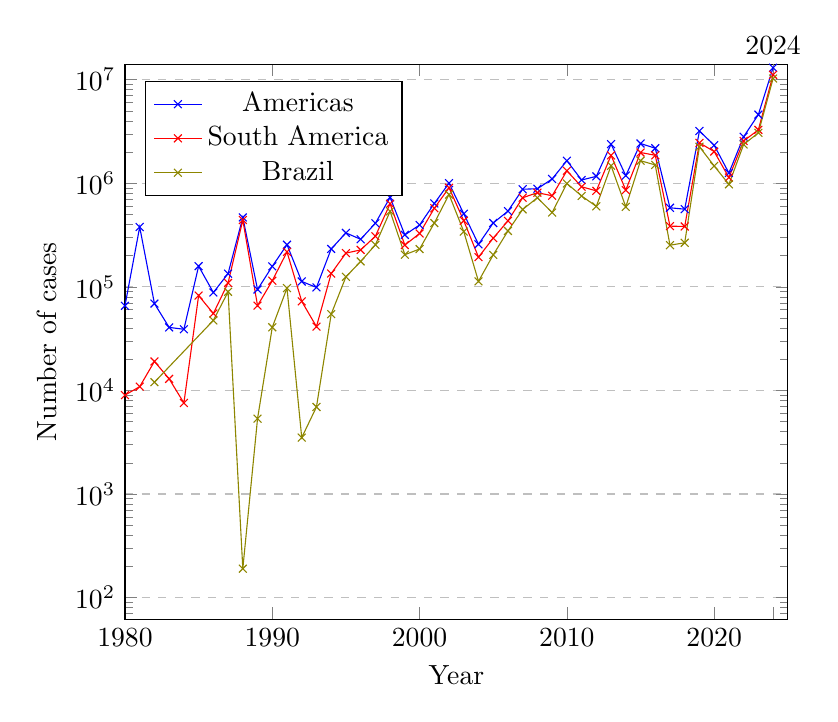
\begin{tikzpicture}[>=latex, scale=1]
		%scale=.6]
		\begin{axis}[
				width = {10cm},
				%title={Dengue reported cases from 1980 to 2022},
				xlabel={Year},
				ylabel={Number of cases},
				ymode=log,
				xmin=1980, xmax=2025,
				ymin=0, ymax=14000000,
				xtick={1980, 1990, 2000, 2010, 2020, 2024},
				xticklabels={1980, 1990, 2000, 2010, 2020},
				extra x ticks={2024},
				extra x tick labels={2024},  % Labels at top
				extra x tick style={ticklabel pos=upper},
				legend pos=north west,
				ymajorgrids=true,
				grid style=dashed,
			]

			\addplot[
				color=blue,
				mark=x,
			]
			plot coordinates {
					(1980, 65523)
					(1981, 377916)
					(1982, 68892)
					(1983, 40544)
					(1984, 38904)
					(1985, 158193)
					(1986, 88093)
					(1987, 134013)
					(1988, 467386)
					(1989, 94179)
					(1990, 157662)
					(1991, 254749)
					(1992, 112567)
					(1993, 98598)
					(1994, 232051)
					(1995, 331417)
					(1996, 287519)
					(1997, 410392)
					(1998, 729425)
					(1999, 317158)
					(2000, 394857)
					(2001, 636977)
					(2002, 1001073)
					(2003, 506726)
					(2004, 257251)
					(2005, 413122)
					(2006, 537412)
					(2007, 874750)
					(2008, 884334)
					(2009, 1099742)
					(2010, 1648569)
					(2011, 1073990)
					(2012, 1164366)
					(2013, 2384803)
					(2014, 1184045)
					(2015, 2416018)
					(2016, 2175409)
					(2017, 579027)
					(2018, 561689)
					(2019, 3190778)
					(2020, 2326115)
					(2021, 1254648)
					(2022, 2811433)
					(2023, 4594823)
					(2024, 13036652)
				};
			\addlegendentry{Americas}

			\addplot[
				color=red,
				mark=x,
			]
			plot coordinates {
					(1980, 9003)
					(1981, 10861)
					(1982, 19034)
					(1983, 12925)
					(1984, 7560)
					(1985, 82273)
					(1986, 55248)
					(1987, 108955)
					(1988, 441382)
					(1989, 65803)
					(1990, 114431)
					(1991, 217077)
					(1992, 72319)
					(1993, 41250)
					(1994, 134342)
					(1995, 211396)
					(1996, 226960)
					(1997, 307625)
					(1998, 632804)
					(1999, 252762)
					(2000, 326846)
					(2001, 572876)
					(2002, 903891)
					(2003, 434264)
					(2004, 193334)
					(2005, 294943)
					(2006, 432661)
					(2007, 724077)
					(2008, 810134)
					(2009, 756755)
					(2010, 1317801)
					(2011, 923793)
					(2012, 843840)
					(2013, 1857228)
					(2014, 857983)
					(2015, 1978921)
					(2016, 1860466)
					(2017, 385076)
					(2018, 382243)
					(2019, 2453060)
					(2020, 2021272)
					(2021, 1134555)
					(2022, 2558083)
					(2023, 3274879)
					(2024, 11118085)
				};
			\addlegendentry{South America}

			\addplot[
				color=olive,
				mark=x,
			]
			plot coordinates {
					(1980, 0)
					(1981, 0)
					(1982, 12000)
					(1983, 0)
					(1984, 0)
					(1985, 0)
					(1986, 47367)
					(1987, 89393)
					(1988, 190)
					(1989, 5334)
					(1990, 40642)
					(1991, 97209)
					(1992, 3501)
					(1993, 6915)
					(1994, 54453)
					(1995, 124775)
					(1996, 175749)
					(1997, 254074)
					(1998, 535283)
					(1999, 204131)
					(2000, 231412)
					(2001, 412388)
					(2002, 778037)
					(2003, 341189)
					(2004, 112851)
					(2005, 203356)
					(2006, 345922)
					(2007, 558413)
					(2008, 724427)
					(2009, 520660)
					(2010, 994158)
					(2011, 753487)
					(2012, 597450)
					(2013, 1473645)
					(2014, 591080)
					(2015, 1649008)
					(2016, 1500535)
					(2017, 252054)
					(2018, 265934)
					(2019, 2248570)
					(2020, 1467142)
					(2021, 975474)
					(2022, 2363490)
					(2023, 3064739)
					(2024, 10239883)
				};
			\addlegendentry{Brazil}
		\end{axis}
	\end{tikzpicture}
	\caption{Dengue reported cases from 1980 to 2024~\citep{paho-1}.}
	\label{fig:dengue_reported_cases_graphic}
\end{figure}

The disease imposes substantial social and economic burdens, affecting not only
the health and well-being of individuals but also the broader economic
productivity and healthcare system. The financial impact of Dengue in Brazil is
profound, for example, annual expenditures on Dengue prevention and control
exceed BRL $1.6$ billion~\citep{negreiros-2020}. The direct costs include
healthcare expenses for hospitalization, medical treatment, and public health
campaigns aimed at controlling mosquito populations~\citep{negreiros:2008}.
Indirect costs, such as lost productivity due to illness and the long-term
effects of severe Dengue cases, add to the financial strain. Moreover, the
social consequences are equally alarming, with communities enduring the
disruption of daily life, increased anxiety over disease outbreaks, and the loss
of lives.

Despite the severity of the situation, most Brazilian municipalities continue to
make crucial decisions in combating Dengue without the support of advanced
computational tools~\citep{brasil-dept-helth:2009}. The current approach is
largely reactive, relying on traditional mosquito control methods, including
eliminating adult mosquitoes, their breeding sites and public health
interventions. These actions are often insufficient to address the complexity
and scale of the problem. This lack of computational support means that
decisions regarding resource allocation, strategic planning, and the deployment
of interventions are not optimized, leading to possible inefficiencies and
potentially exacerbating the spread of the
disease~\citep{forbes-2002,xie-2015,rais-2011}.

The most common approach to combating Dengue spread is employing chemical
control methods, such as insecticides, which manage the mosquito population in
both the larval and adult stages~\citep{brasil-dept-helth:2009}. The \gls{who}
provides technical and operational standards for pesticide experts to ensure the
safe use of insecticides in public health. These standards specify the active
ingredients and dosages for various treatments. During disease outbreaks,
emergency responses in urban areas usually involve the dispatch of spraying
vehicles to apply insecticides (see Figure~\ref{fig:nebulizer}). It is essential
to use insecticides carefully and responsibly in vector control activities, as
indiscriminate use can have significant environmental impacts and contribute to
developing resistance in mosquitoes~\citep{WHO2009,WHO2020}.

\begin{figure}[h!]
	\centering
	\includegraphics[scale=0.5]{images/fumace.jpg}
	\caption{Nebulizer equipment attached to vehicle \citep{fumace-2022}.}
	\label{fig:nebulizer}
\end{figure}

The sprayed insecticide has no residual  effect and it is strongly influenced by
wind  and obstacles  along the  streets. The  best effect  is achieved  when the
densest  insecticide cloud  is at  a distance  of at  most 100  meters from  the
equipment~\citep{brasil-dept-helth:2009}.  As this  distance  is  crossed, the
effectiveness  decreases, as a consequence of droplet drift influenced by
factors of the environment. The cloud dispersion is illustrated in
Figure~\ref{fig:dispersion}.

\begin{figure}[!ht]
	\centering
	\includegraphics[scale=0.4]{images/cloud-dispersion.png}
	\caption{Cloud dispersion of the application \citep{brasil-dept-helth:2009}.}
	\label{fig:dispersion}
\end{figure}

Insecticide application instructions are generally based on ideal topology
conditions, locality structure, and favorable winds. The operation is often
affected by unpaved roads, the presence of high walls,  and  high   vegetation,
in  addition  to   headwinds.  The application methodology must consider these
limitations to obtain a good impact on the vector population. Once a spraying
vehicle begins to service a city block, it must sequentially cover all
surrounding streets in a clockwise direction. The traversal ensures that the
insecticide fog forms a continuous barrier, preventing mosquitoes from escaping.
The clockwise direction is due to real operational factors, as the nebulizer
equipment points to the right side of the vehicle.

Figure~\ref{fig:instance_digraph_fumace_car} shows an example of a map, with
four blocks to service, and Figure~\ref{fig:route_fumace_car} presents a
spraying route for these blocks where the nebulizer is activated in the black
dots and follows the direction of the arrow, starts by serving Block 2, goes to
Blocks 1, 3 and 4, respectively.

\begin{figure}[!ht]
	\begin{minipage}[c]{.49\textwidth}
		\centering
		\subfloat[Street blocks example.]{\label{fig:instance_digraph_fumace_car}\includegraphics[width=5cm, height=5cm]{images/cbrp-instance.pdf}} \end{minipage}%
	\begin{minipage}[c]{.49\textwidth}
		\centering
		\subfloat[Spraying route example.]{\label{fig:route_fumace_car}\includegraphics[width=8cm, height=5cm]{images/nebulizer-activated.pdf}}
	\end{minipage}
	\caption{Vehicle pattern with nebulizer \cite{brasil-dept-helth:2009}.}
\end{figure}

As a result, health authorities with limited budgets must make two key
decisions: first, selecting which city blocks should receive insecticide
spraying to maximize vector suppression; and second, optimizing vehicle routes
to ensure the efficient use of available resources. In this context, there is a
clear and urgent need to integrate computational models and decision-support
systems into Dengue control strategies. Such tools can help municipalities
better predict outbreaks, optimize resource use, and implement more effective
mosquito control measures.

In operations research, routing problems are typically classified based on where
the service is performed. When services are provided at specific locations
(nodes), they fall under \gls{vrp}~\citep{braekers2016vehicle}. When services
are conducted along edges (or arcs), they are categorized as
\gls{arp}~\citep{corberan2021arc}. The routing challenge in Dengue control
exhibits the characteristics of both \gls{vrp} and \gls{arp}. Each city block
can be represented as a \textit{super-node} (similar to a \gls{vrp}), while
spraying occurs along the surrounding arcs, aligning with \gls{arp} features.
Given this hybrid structure, we introduce and explore a new problem, titled the
\gls{cbrp}.

The \gls{cbrp} aims to optimize the servicing of city blocks within an urban
street network by assigning spraying vehicles. However, due to limited
operational resources, only a subset of city blocks can be serviced. A city
block is considered serviced if a spraying vehicle completely encircles it
without detours, and each serviced block contributes a predefined benefit. Thus,
the primary objective of the \gls{cbrp} is to identify the subset of blocks
whose servicing yields the highest aggregate benefit, alongside determining the
optimal vehicle routes to achieve this objective within the available resources.

The Figure~\ref{fig:ex1} illustrates an example of an input graph (city map) and
a corresponding \gls{cbrp} feasible solution. In Figure~\ref{subfig:a}, the
circles represent the graph nodes, while the labels from A to H indicate the
city blocks. Figure~\ref{subfig:b} depicts a feasible solution to the
\gls{cbrp}. In this solution, the nodes used in the route are marked as squares
and connected by black arrows (nodes 4, 5, 3, and 9). Squares with a double
border denote nodes that act as starting points to serve at least one block. The
atended blocks are represented by the arcs connected to the double square with
the same color, for example: node 4 (blue) serves blocks A (arcs
4$\rightarrow$8, 8$\rightarrow$1 and 1$\rightarrow$4) and B (arcs
4$\rightarrow$6, 6$\rightarrow$8 and 8$\rightarrow$4). Node 5 (red) serves
blocks D and F, node 3 does not serve any block, and node 9 (teal) serves block
H.

\begin{figure}[!ht]
	\begin{subfigure}{.5\textwidth}
		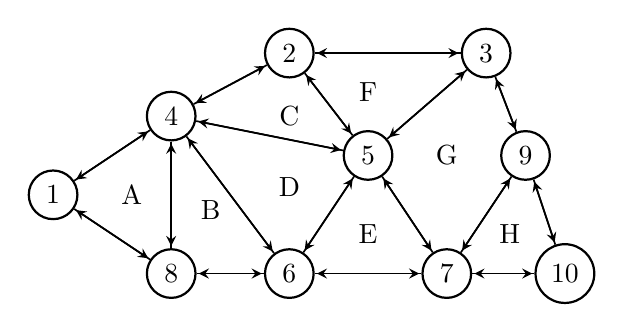
\begin{tikzpicture}[
				> = stealth, % arrow head style
				shorten > = 0.8pt, % don't touch arrow head to node
				auto,
				node distance = 1cm, % distance between nodes
				semithick % line style
			]

			\tikzstyle{every state}=[
			draw = black,
			thick,
			fill = white,
			minimum size = 5mm
			]

			\node[state] (a) [at={(-1, -0.5)}]{$1$};
			\node[state] (b) [at={(2,1.3)}] {$2$};
			\node[state] (c) [at={(4.5,1.3)}] {$3$};
			\node[state] (d) [at={(0.5, 0.5)}] {$4$};
			\node[state] (e) [at={(3, 0)}] {$5$};
			\node[state] (f) [at={(2,-1.5)}] {$6$};
			\node[state] (g) [at={(4,-1.5)}] {$7$};
			\node[state] (i) [at={(0.5,-1.5)}] {$8$};
			\node[state] (j) [at={(5,0)}] {$9$};
			\node[state] (k) [at={(5.5,-1.5)}] {$10$};
			% Blocks
			\node[state, draw = white, right of = a] {A};
			\node[state, draw = white, right of = i, yshift=0.8cm, xshift=-0.5cm] {B};
			\node[state, draw = white, below of = b, yshift=0.2cm] {C};
			\node[state, draw = white, left of = e, yshift=-0.4cm] {D};
			\node[state, draw = white, below of = e] {E};
			\node[state, draw = white, right of = b, yshift=-0.5cm] {F};
			\node[state, draw = white, right of = e] {G};
			\node[state, draw = white, below of = j, xshift=-0.2cm] {H};


			\path[->] (a) edge node {} (d);
			\path[->] (d) edge node {} (a);
			\path[->] (i) edge node {} (a);
			\path[->] (a) edge node {} (i);
			\path[->] (b) edge node {} (d);
			\path[->] (d) edge node {} (b);
			\path[->] (b) edge node {} (c);
			\path[->] (c) edge node {} (b);
			\path[->] (c) edge node {} (e);
			\path[->] (e) edge node {} (c);
			\path[->] (e) edge node {} (f);
			\path[->] (f) edge node {} (e);
			\path[->] (d) edge node {} (i);
			\path[->] (i) edge node {} (d);
			\path[->] (d) edge node {} (e);
			\path[->] (e) edge node {} (d);
			\path[->] (d) edge node {} (f);
			\path[->] (f) edge node {} (d);
			\path[->] (e) edge node {} (g);
			\path[->] (g) edge node {} (e);
			\path[->] (c) edge node {} (j);
			\path[->] (j) edge node {} (c);
			\path[->] (i) edge node {} (f);
			\path[->] (f) edge node {} (i);
			\path[->] (j) edge node {} (k);
			\path[->] (k) edge node {} (j);
			\path[->] (j) edge node {} (g);
			\path[->] (g) edge node {} (j);
			\path[->] (e) edge node {} (b);
			\path[->] (b) edge node {} (e);
			\path[->] (f) edge node {} (g);
			\path[->] (g) edge node {} (f);
			\path[->] (g) edge node {} (k);
			\path[->] (k) edge node {} (g);

		\end{tikzpicture}
		\subcaption{\label{subfig:a} Initial graph and blocks.}
	\end{subfigure}
	% Segunda figura
	\begin{subfigure}{.5\textwidth}
		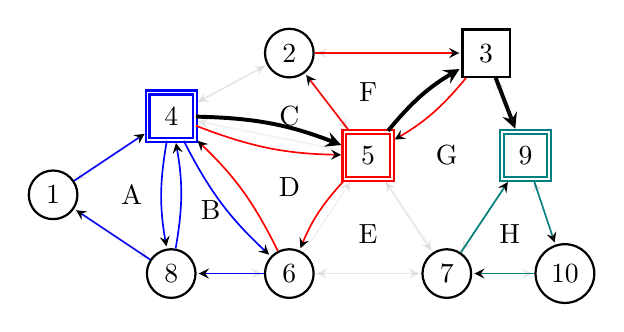
\begin{tikzpicture}[
				> = stealth, % arrow head style
				shorten > = 0.8pt, % don't touch arrow head to node
				auto,
				node distance = 1cm, % distance between nodes
				semithick % line style
			]

			\tikzstyle{every state}=[
			draw = black,
			thick,
			fill = white,
			minimum size = 6mm
			]

			\node[state] (a) [at={(-1, -0.5)}]{$1$};
			\node[state] (b) [at={(2,1.3)}] {$2$};
			\node[state, rectangle] (c) [at={(4.5,1.3)}] {$3$};
			\node[state, rectangle, double, draw=blue] (d) [at={(0.5, 0.5)}] {$4$};
			\node[state, rectangle, double, draw=red] (e) [at={(3, 0)}] {$5$};
			\node[state] (f) [at={(2,-1.5)}] {$6$};
			\node[state] (g) [at={(4,-1.5)}] {$7$};
			\node[state] (i) [at={(0.5,-1.5)}] {$8$};
			\node[state, rectangle, double, draw=teal] (j) [at={(5,0)}] {$9$};
			\node[state] (k) [at={(5.5,-1.5)}] {$10$};
			% Blocks
			\node[state, thick, dashed, draw = white, right of = a] {A};
			\node[state, thick, dashed, draw = white, right of = i, yshift=0.8cm, xshift=-0.5cm] {B};
			\node[state, draw = white, below of = b, yshift=0.2cm] {C};
			\node[state, thick, dashed, draw = white, left of = e, yshift=-0.4cm] {D};
			\node[state, draw = white, below of = e] {E};
			\node[state, thick, dashed, draw = white, right of = b, yshift=-0.5cm] {F};
			\node[state, draw = white, right of = e] {G};
			\node[state, thick, dashed, draw = white, below of = j, xshift=-0.2cm] {H};
			% Dummy
			%\node[state, double, above of = a] (s) {s};
			%\node[state, double, right of = j, xshift=0.2cm] (t) {t};
			%\path[->, draw = black, opacity = 1.0] (s) edge node {} (d);
			%\path[->, draw = black, opacity = 1.0] (j) edge node {} (t);

			\path[->, draw = blue, opacity = 1.0] (a) edge node {} (d);
			\path[->, draw = gray, opacity = 0.1] (d) edge node {} (a);
			\path[->, draw = blue, opacity = 1.0] (i) edge node {} (a);
			\path[->, draw = gray, opacity = 0.1] (a) edge node {} (i);
			\path[->, draw = gray, opacity = 0.1] (b) edge node {} (d);
			\path[->, draw = gray, opacity = 0.1] (d) edge node {} (b);
			\path[->, draw = red, opacity = 1.0] (b) edge node {} (c);
			\path[->, draw = gray, opacity = 0.1] (c) edge node {} (b);
			\path[->, draw = red, opacity = 1.0, bend left=10] (c) edge node {} (e);
			\path[->, draw = black, opacity = 1.0, bend left=10, line width=0.5mm] (e) edge node {} (c);
			\path[->, draw = red, opacity = 1.0, bend right=10] (e) edge node {} (f);
			\path[->, draw = gray, opacity = 0.1] (f) edge node {} (e);
			\path[->, draw = blue, opacity = 1.0, bend right=10] (d) edge node {} (i);
			\path[->, draw = blue, opacity = 1.0, bend right=10] (i) edge node {} (d);
			\path[->, draw = black, opacity = 1.0, bend left=10, line width=0.5mm] (d) edge node {} (e);
			\path[->, draw = red, opacity = 1.0, bend right=10] (d) edge node {} (e);
			\path[->, draw = gray, opacity = 0.1] (e) edge node {} (d);
			\path[->, draw = blue, opacity = 1.0, bend right=10] (d) edge node {} (f);
			\path[->, draw = red, opacity = 1.0, bend right=10] (f) edge node {} (d);
			\path[->, draw = gray, opacity = 0.1] (e) edge node {} (g);
			\path[->, draw = gray, opacity = 0.1] (g) edge node {} (e);
			\path[->, draw = black, opacity = 1.0, line width=0.5mm] (c) edge node {} (j);
			\path[->, draw = gray, opacity = 0.1] (j) edge node {} (c);
			\path[->, draw = gray, opacity = 0.1] (i) edge node {} (f);
			\path[->, draw = blue, opacity = 1.0] (f) edge node {} (i);
			\path[->, draw = teal, opacity = 1.0] (j) edge node {} (k);
			\path[->, draw = gray, opacity = 0.1] (k) edge node {} (j);
			\path[->, draw = gray, opacity = 0.1] (j) edge node {} (g);
			\path[->, draw = gray, opacity = 0.1] (g) edge node {} (j);
			\path[->, draw = red, opacity = 1.0] (e) edge node {} (b);
			\path[->, draw = gray, opacity = 0.1] (b) edge node {} (e);
			\path[->, draw = gray, opacity = 0.1] (f) edge node {} (g);
			\path[->, draw = gray, opacity = 0.1] (g) edge node {} (f);
			\path[->, draw = gray, opacity = 0.1] (g) edge node {} (k);
			\path[->, draw = teal, opacity = 1.0] (k) edge node {} (g);
			\path[->, draw = teal, opacity = 1.0] (g) edge node {} (j);
		\end{tikzpicture}
		\subcaption{\label{subfig:b} Route and attended blocks.}
	\end{subfigure}
	\caption{\label{fig:ex1} CBRP instance (a) and solution (b).}
\end{figure}

Given the complex and dynamic nature of urban environments, particularly in
public health scenarios like Dengue control, incorporating stochastic elements
into the \gls{cbrp} is essential to enhance the realism and applicability of the
solution. Some unpredictable behavior of mosquitoes and the spread of Dengue
cases during seasons of the years highlight the need for a stochastic version of
the \gls{cbrp}. This leads to solutions that better reflect the variability of
actual deployment scenarios, improving the adherence of the model to real-world
challenges. Moreover, by accounting for probabilistic factors, stochastic
approaches can prioritize the most critical city blocks under uncertain resource
availability, thereby increasing the effectiveness and resilience of vector
control interventions.

The \gls{cbrp} extends beyond its application in vector control, providing a
robust framework to address a variety of urban logistics challenges. These
challenges include waste collection, postal delivery, and reading of utility
meters, where the primary goal is to efficiently service city blocks while
managing both spatial and resource constraints. The flexibility of the
\gls{cbrp} makes it particularly valuable in densely populated urban
environments, where the efficiency of routing decisions significantly affects
both service effectiveness and operational costs.

Besides the definition of control actions~\citep{gomez-2009,jing2019dengue}, it
is important to develop visualization and decision support tools to assist the
health departments. A clear understanding of the likely progression of Dengue
cases can significantly enhance short-term resource allocation
strategies~\citep{brasil-dept-helth:2009}. Generating accurate predictive models
for Dengue spread, especially in urban areas is highly challenging since
mosquito behavior is inconsistent and depends on numerous factors. These include
the availability and location of breeding sites, the mosquito population size
and infection rate, the timing and location of insecticide application,
frequency of rainfall, various climate conditions, and the interactions between
mosquitoes, breeding sites, and human populations.

In this thesis, we developed a complete set of methodologies focused in the
application of \gls{cbrp} to optimize insecticide-spraying routes for Dengue
control. Those methodologies compreend exact and heuristic approaches for
deterministic and stochastic versions of the \gls{cbrp}, instances based on real
data, robust simulation based on multi-agent systems and a
simulation-optimization framework that could assist health departments. This
application is particularly pertinent to many Brazilian cities, where seasonal
outbreaks of mosquito-borne diseases demand resource-efficient, targeted vector
control strategies. By optimizing spray routes, the \gls{cbrp} not only improves
operational efficiency but also maximizes coverage of high-risk areas,
ultimately supporting public health initiatives aimed at reducing Dengue
transmission.

% The \gls{mabs} have become increasingly popular in various fields due to their
% ability to capture the complexity and dynamics of real-world
% systems~\citep{siebers-2008}. Unlike traditional simulations that rely on a set
% of predetermined rules and assumptions, multi-agent simulations allow for
% interactions between agents to emerge organically, leading to the emergence of
% unexpected and emergent behaviors. This makes them an effective tool for
% understanding and predicting the behavior of complex systems, such as social and
% economic systems, ecological systems, and even biological
% systems~\citep{ballet-2020}. Additionally, multi-agent simulations provide a
% flexible and adaptable approach that can be easily modified and scaled to
% simulate different scenarios and environments. With the increasing availability
% of computing resources, multi-agent simulations have become an important tool
% for modeling and simulating complex systems, providing valuable insights into
% the behavior and evolution of these systems~\citep{selvaratnam-1995}.


%\paragraph{Our contributions.} The contributions of this study are three-fold.
% First, it advances vector control strategies by proposing novel methodologies
% for the optimal routing of spraying vehicles. Our approaches are based on
% mixed-integer linear programming (MILP) formulations and biased-random key
% genetic algorithms (BRKGA). Second, we introduce a systematic procedure for
% generating realistic problem instances by mapping city blocks and their
% surrounding street arcs. Third, through extensive computational experiments
% utilizing seven years of Dengue case data from two Brazilian cities, we
% demonstrate that our proposed methodologies significantly improve vector
% control effectiveness, potentially reducing Dengue transmission rates and
% improving public health outcomes. These findings offer valuable insights to
% public health authorities, policymakers, and researchers working on complex
% vector-borne disease challenges. Moreover, the generality of the CBRP
% framework makes it a promising approach for optimizing vehicle routing
% strategies in other city-block service applications.

% \paragraph{Text organization.}
% The remainder of this thesis is organized as follows.
% Chapter~\ref{chp:preliminary-concepts} formally defines the City Block Routing Problem (CBRP).
% Chapter~\ref{chp:literature_review} reviews existing operations research, \gls{ml} and simulation approaches relevant to Dengue vector control.
% Section~\ref{sec:models} introduces and describes the proposed mathematical formulations for the CBRP.
% Section~\ref{sec:data} explains the datasets and experimental setups employed to evaluate the proposed methodologies.
% Section~\ref{sec:results} discusses computational results and assesses the methodologies' performance.
% Finally, Section~\ref{sec:conclusions} summarizes the findings and provides concluding remarks.
\chapter{Preliminary Concepts and Formulations}\label{chp:preliminary-concepts}

In this chapter, we introduce the fundamental concepts necessary for
understanding this thesis. The basic notation and definitions are presented in
Section~\ref{sec:not-e-def}. In this work, we employ basic concepts from
Combinatorial Optimization, which are assumed to be known. If the reader deems a
review necessary, we recommend the textbook by Nemhauser and
Wolsey~\cite{Nemhauser}, which covers this topic with a focus on \gls{ilp}, one
of the main tools used in this work. Basic concepts related to graph theory are
also assumed to be known. Should the
reader require a refresher, the material can be found in standard textbooks on
the subject, such as Diestel~\cite{diestel:2005}. 

% TODO: add references to the sections
% The mathematical models are presented in Sections~\ref{sec:dmfm-pma}
% and~\ref{sec:ab-pma}. Section~\ref{sec:rel-lagrangiana} provides a description
% of the functioning and application of Lagrangian relaxation, one of the main
% approaches employed in this work. Finally, in Sections~\ref{sec:metaheuristic}
% and~\ref{subsec:brkga}, we present a general discussion on metaheuristics.


\section{Notations and Definitions}\label{sec:not-e-def}

Once a spraying vehicle begins to service a city block, it must sequentially
cover all surrounding edges in a clockwise direction. The
traversal ensures that the insecticide fog forms a continuous barrier,
preventing mosquitoes from escaping. 
The clockwise direction is due to real operational factors, 
as the nebulizer equipment points to the right side of the
vehicle. 
Figure~\ref{fig:instance_digraph_fumace_car} shows an example of a map,
with four blocks to service, and Figure~\ref{fig:route_fumace_car} presents a
spraying route for these blocks where the nebulizer is activated in the black
dots and follows the direction of the arrow, starts by serving Block 2, goes to
Blocks 1, 3 and 4, respectively. 

\begin{figure}[!ht]
	\begin{minipage}[c]{.49\textwidth}
		\centering
		\subfloat[A CBRP instance
			digraph.]{\label{fig:instance_digraph_fumace_car}\includegraphics[width=5cm,
				height=5cm]{images/cbrp-instance.pdf}} \end{minipage}%
	\begin{minipage}[c]{.49\textwidth}
		\centering
		\subfloat[A spraying vehicle route covering four city
			blocks.]{\label{fig:route_fumace_car}\includegraphics[width=8cm,
				height=5cm]{images/nebulizer-activated.pdf}}
	\end{minipage}
	\caption{\label{fig:route-ex} CBRP example.}
\end{figure}


Let $G = (V, A, B)$ be a weighted and directed graph, where $V = \{1, \dots, n\}$
is the set of vertices, $A = \{(i, j) : i, j \in V, i \neq j\}$
is the set of $m$ arcs, and $B = \{b : b \subseteq V\}$ is the set of blocks.
In each arc, the first vertex is the source and also the
predecessor of the second vertex in the ordered pair, which is known as the
destination. Each block $b$ has an associated set of arcs $B(i, j) \subseteq A$ that
can be serviced by a vehicle. 

We now present a formal definition of the \gls{cbrp}. Let a Plannar Graph,
extracted from a real citymap, be represented as a weighted directed graph
$G$. Each node in $V$ represents the intersection of at least two
streets and has a list of blocks $b \subseteq B$ that are associated with it.
Each arc $(i, j) \in A$ has a deadheading time $t_{i, j} > 0$, a service time
$t^{'}_{i, j} > 0$ such that $t_{i, j} \leqslant t^{'}_{i, j}$ and the block
$b \in B$ that is associated with it. The input to the \gls{cbrp} is defined as:

\begin{itemize}
	\item $G = (V, A, B)$ is a weighted directed planar graph with the blocks associated with it;
	\item $p_b : B \rightarrow \mathbb{N}$ is a function that returns the profit
	      for each block $b \in B$;
	\item $t_{i, j} : A \rightarrow \mathbb{N}$ is a function that returns the
	      deadheading time for each arc $(i, j) \in A$;
	\item $t^{'}_{i, j} : A \rightarrow \mathbb{N}$ is a function that returns
	      the service time for each arc $(i, j) \in A$;
	\item $T$ is the time limit for the vehicle to travel and service the blocks;
	\item $V(b)$ is the set of nodes that are associated with the block $b \in B$;
	\item $B(i)$ is the set of blocks that are associated with the node $i \in V$;
	\item $B(i, j)$ is the set of blocks that are associated with the arc $(i, j) \in A$;
	\item $\delta^{+}_{i}$ is the set of arcs with destination $i$;
	\item $\delta^{-}_{i}$ is the set of arcs with source $i$;
\end{itemize}

The \gls{cbrp} is introduced as a general framework for addressing the routing of
spraying vehicles and other city block servicing problems. 
The objective of the \gls{cbrp} is to determine an optimal traversal that 
services a subset of blocks within a network, maximizing the total 
collected benefit from each serviced block. 
A vehicle traverses the graph $G$ following a route that can serve a
subset of blocks within a given time limit $T$. This work considers two types of 
solution routes, depending on whether the vertices can be
visited more than once: \textit{Walk-based route}, in which any vertex (or arc)
can be visited multiple times and \textit{Path-based route}, in which no vertex
appears more than once. 
An optimal route (walk or path) is one that maximizes
the total prize collected from the serviced blocks while respecting the vehicle
time limit $T$.

To facilitate modeling, we augment the graph $G$ by introducing a dummy depot
$0$, from which the route originates, and a set of arcs $\{(0, i), (i, 0) :
	\forall i \in V\}$ with times $t_{i,0} = t_{0,i} = 0$, $\forall i \in V$. 
Thus, we define the modified graph as $G' = (V' = V \cup \{0\}, A' = A \cup \{(0,
	i), (i, 0) : \forall i \in V\})$.

We now present key properties of the \gls{cbrp}. First, due to the operational
restrictions, once a block $b$ starts being serviced at a given node $i$, it
must be fully encircled before the vehicle moves to another block. This leads
to the following property:

\begin{property}
	\label{claim:core_insight}
	A block can be serviced if at least one of its nodes is visited.
\end{property}

From Property~\ref{claim:core_insight}, 
when formulating the problem, it is not
necessary to explicitly require the vehicle to completely traverse a block's
perimeter in order to count it as serviced. Instead, servicing can be achieved
by visiting at least one node within the block and accounting for the
corresponding service time. This property is valid due to the definition of the blocks $B$ and
the fact that the vehicle must service all blocks in a clockwise direction.

Figure~\ref{fig:servicing_block_no_surrounding_strategy} illustrates an example of
this strategy, where servicing is achieved without requiring a full traversal of
the block's perimeter.

\begin{figure}[!ht]
	\begin{minipage}[c]{.32\textwidth}
		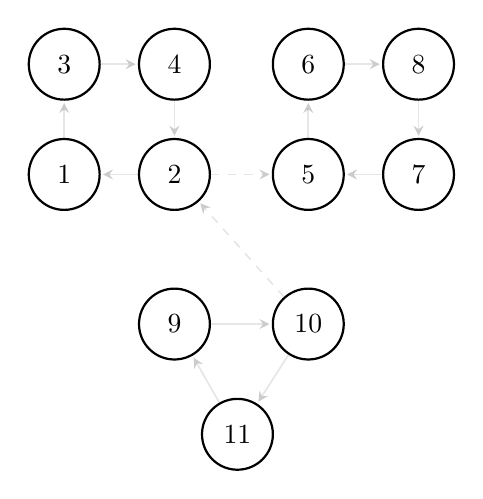
\begin{tikzpicture}[
				> = stealth, % arrow head style
				shorten > = 0.8pt, % don't touch arrow head to node
				auto,
				node distance = 1.4cm, % distance between nodes
				semithick % line style
			]
			
			\tikzstyle{every state}=[
			draw = black,
			thick,
			fill = white,
			minimum size = 9mm
			]
			
			\node[state] (a) at (0,0) {$1$};
			\node[state, right of = a] (b) {$2$};
			\node[state, above of = a] (c) {$3$};
			\node[state, above of = b] (d) {$4$};
			
			\node[state, right of = b, xshift=0.3cm] (e) {$5$};
			\node[state, right of = d, xshift=0.3cm] (f) {$6$};
			\node[state, right of = e] (g) {$7$};
			\node[state, right of = f] (h) {$8$};
			
			\node[state, below of = b, yshift=-0.5cm] (i) {$9$};
			\node[state, below of = e, yshift=-0.5cm] (j) {$10$};
			\node[state, below of = i, left of = j, xshift=0.5cm] (k) {$11$};
			
			\path[->, draw = gray, opacity = 0.2] (a) edge node {} (c); 
			\path[->, draw = gray, opacity = 0.2] (c) edge node {} (d); 
			\path[->, draw = gray, opacity = 0.2] (d) edge node {} (b);
			\path[->, draw = gray, opacity = 0.2] (b) edge node {} (a);
			
			\path[->, draw = gray, opacity = 0.2] (e) edge node {} (f);
			\path[->, draw = gray, opacity = 0.2] (f) edge node {} (h);
			\path[->, draw = gray, opacity = 0.2] (h) edge node {} (g);
			\path[->, draw = gray, opacity = 0.2] (g) edge node {} (e);
			
			\path[->, draw = gray, opacity = 0.2] (i) edge node {} (j);
			\path[->, draw = gray, opacity = 0.2] (j) edge node {} (k);
			\path[->, draw = gray, opacity = 0.2] (k) edge node {} (i);
			
			\path[->, draw = gray, opacity = 0.2, dashed] (j) edge node {} (b);
			\path[->, draw = gray, opacity = 0.2, dashed] (b) edge node {} (e);
		\end{tikzpicture}
		\subcaption{Instance Example.}
	\end{minipage}
	\hfill
	\begin{minipage}[c]{.32\textwidth}
		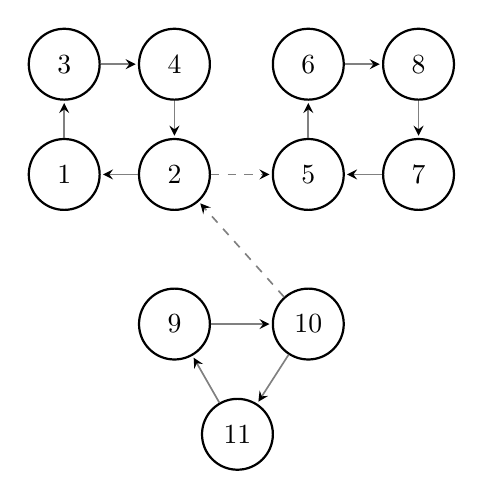
\begin{tikzpicture}[
				> = stealth, % arrow head style
				shorten > = 0.8pt, % don't touch arrow head to node
				auto,
				node distance = 1.4cm, % distance between nodes
				semithick % line style
			]
			
			\tikzstyle{every state}=[
			draw = black,
			thick,
			fill = white,
			minimum size = 9mm
			]
			
			\node[state] (a) at (0,0) {$1$};
			\node[state, right of = a] (b) {$2$};
			\node[state, above of = a] (c) {$3$};
			\node[state, above of = b] (d) {$4$};
			
			\node[state, right of = b, xshift=0.3cm] (e) {$5$};
			\node[state, right of = d, xshift=0.3cm] (f) {$6$};
			\node[state, right of = e] (g) {$7$};
			\node[state, right of = f] (h) {$8$};
			
			\node[state, below of = b, yshift=-0.5cm] (i) {$9$};
			\node[state, below of = e, yshift=-0.5cm] (j) {$10$};
			\node[state, below of = i, left of = j, xshift=0.5cm] (k) {$11$};
			
			\path[->, draw = gray, opacity = 1.0] (a) edge node {} (c); 
			\path[->, draw = gray, opacity = 1.0] (c) edge node {} (d); 
			\path[->, draw = gray, opacity = 1.0] (d) edge node {} (b);
			\path[->, draw = gray, opacity = 1.0] (b) edge node {} (a);
			
			\path[->, draw = gray, opacity = 1.0] (e) edge node {} (f);
			\path[->, draw = gray, opacity = 1.0] (f) edge node {} (h);
			\path[->, draw = gray, opacity = 1.0] (h) edge node {} (g);
			\path[->, draw = gray, opacity = 1.0] (g) edge node {} (e);
			
			\path[->, draw = gray, opacity = 1.0] (i) edge node {} (j);
			\path[->, draw = gray, opacity = 1.0] (j) edge node {} (k);
			\path[->, draw = gray, opacity = 1.0] (k) edge node {} (i);
			
			\path[->, draw = gray, opacity = 1.0, dashed] (j) edge node {} (b);
			\path[->, draw = gray, opacity = 1.0, dashed] (b) edge node {} (e);
		\end{tikzpicture}
		\subcaption{Explicity Block Servicing.}
	\end{minipage}\\
	\centering
	\begin{minipage}[c]{.32\textwidth}
		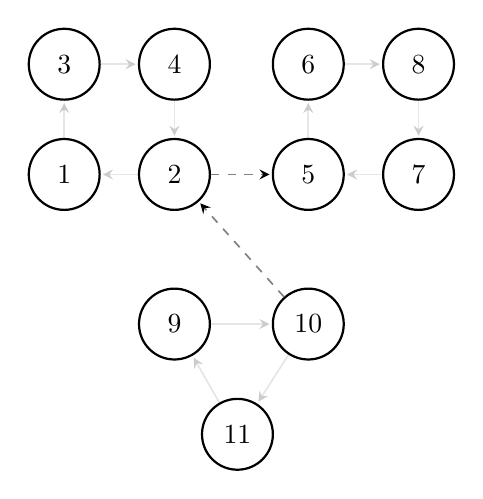
\begin{tikzpicture}[
				> = stealth, % arrow head style
				shorten > = 0.8pt, % don't touch arrow head to node
				auto,
				node distance = 1.4cm, % distance between nodes
				semithick % line style
			]
			
			\tikzstyle{every state}=[
			draw = black,
			thick,
			fill = white,
			minimum size = 9mm
			]
			
			\node[state] (a) at (0,0) {$1$};
			\node[state, right of = a] (b) {$2$};
			\node[state, above of = a] (c) {$3$};
			\node[state, above of = b] (d) {$4$};
			
			\node[state, right of = b, xshift=0.3cm] (e) {$5$};
			\node[state, right of = d, xshift=0.3cm] (f) {$6$};
			\node[state, right of = e] (g) {$7$};
			\node[state, right of = f] (h) {$8$};
			
			\node[state, below of = b, yshift=-0.5cm] (i) {$9$};
			\node[state, below of = e, yshift=-0.5cm] (j) {$10$};
			\node[state, below of = i, left of = j, xshift=0.5cm] (k) {$11$};
			
			\path[->, draw = gray, opacity = 0.2] (a) edge node {} (c); 
			\path[->, draw = gray, opacity = 0.2] (c) edge node {} (d); 
			\path[->, draw = gray, opacity = 0.2] (d) edge node {} (b);
			\path[->, draw = gray, opacity = 0.2] (b) edge node {} (a);
			
			\path[->, draw = gray, opacity = 0.2] (e) edge node {} (f);
			\path[->, draw = gray, opacity = 0.2] (f) edge node {} (h);
			\path[->, draw = gray, opacity = 0.2] (h) edge node {} (g);
			\path[->, draw = gray, opacity = 0.2] (g) edge node {} (e);
			
			\path[->, draw = gray, opacity = 0.2] (i) edge node {} (j);
			\path[->, draw = gray, opacity = 0.2] (j) edge node {} (k);
			\path[->, draw = gray, opacity = 0.2] (k) edge node {} (i);
			
			\path[->, draw = gray, opacity = 1.0, dashed] (j) edge node {} (b);
			\path[->, draw = gray, opacity = 1.0, dashed] (b) edge node {} (e);
		\end{tikzpicture}
		\subcaption{Implicit Block Servicing.}
	\end{minipage}
	\caption{\label{fig:servicing_block_no_surrounding_strategy} Strategies for servicing blocks.}
\end{figure}

\section{Deterministic Models}\label{sec:cbrp-deterministic-models}

Given as instance for the \gls{cbrp}, consider a path-based solution on the
original planar graph, in which no arc or vertex is visited more than once. The
following binary decision variables are introduced for the model:

\begin{itemize}
	\item $x_{ij} \in \{0, 1\}$ is a binary variable that indicates whether the arc $(i, j) \in A'$ is included in the route ($x_{ij} = 1$) or not ($x_{ij} = 0$);
	\item $y_{ib} \in \{0, 1\}$ is a binary variable that indicates whether node $i \in V$ is selected as the starting point for serving block $b \in B(i)$ ($y_{ib} = 1$) or not ($y_{ib} = 0$).
\end{itemize}

The Path-CBRP formulation is defined as follows:

\begin{align}
	\text{(Path-CBRP) }          & \max \sum_{i \in V} \sum_{b \in B} p_b y_{ib}                                             & \label{eq:of}                                                  \\
	\nonumber \text{subject to:} &                                                                                           &                                                                \\
	                             & \sum_{i \in V} x_{0,i} = \sum_{j \in V} x_{j,0} = 1                                       & \label{eq:s-t-all}                                             \\
	%
	                             & \sum_{i \in V} x_{i,j} - \sum_{k \in V} x_{j,k} = 0                                       & \ \forall j \in V \label{eq:flow-conservation}                 \\
	%
	                             & \sum_{i \in V(b)} y_{ib} \leq 1                                                           & \ \forall b \in B \label{eq:max-attend}                        \\
	%
	                             & \sum_{j \in \delta^{-}(i)} x_{i,j} \geq y_{ib}                                            & \ \forall b \in B, i \in V(b) \label{eq:in-path}               \\
	%
	                             & \sum_{(i, j) \in A} x_{i,j}t_{i,j} + \sum_{i \in V} \sum_{b \in B} y_{ib}t^{'}_{b} \leq T & \label{eq:max-time}                                            \\
	                             & \sum_{(i, j) \in A(S)} x_{i,j} \leq |V(S)| - 1                                            & \ \forall S \subseteq V \label{eq:circuit-subtour-elimination} \\	
	                             & x \in \mathbb{B}^{|A'|}                                                                   & \label{eq:dom-x}                                               \\
	                             & y \in \mathbb{B}^{|V'| * |B|}.                                                            & \label{eq:dom-y}
\end{align}


The Path-CBRP formulation generates a closed path that starts and ends at the
depot. The objective function~\eqref{eq:of} maximizes the total prize collected
from each serviced block.
Constraints~\eqref{eq:s-t-all}-\eqref{eq:flow-conservation} enforce the start
and end of the route at the depot, and the flow conservation at each node, i.e.
the number of arcs entering a node equals to the number of arcs leaving it.
Constraints~\eqref{eq:max-attend} and~\eqref{eq:in-path} ensure that exactly one
node is selected as the starting point for servicing a block.
Constraints~\eqref{eq:max-time} impose a time limit, accounting for differences
in time spent while servicing and traveling.
Constraints~\eqref{eq:circuit-subtour-elimination} prevent the
formation of subcycles. Finally, constraints~\eqref{eq:dom-x} and~\eqref{eq:dom-y}
define the domain of the decision variables.

Since the subcycle elimination constraints are exponentially large in relation
to the input size, there are two most common approaches to solve Path-CBRP:
the first is to apply the subcycle elimination procedure to integer solutions
obtained during the solver branch and bound. The second is to replace the
constraint by a more compact set of constraints based on the \gls{mtz}
formulation.

% TODO: move to a future subsection with more details
% The implementation of the subtour elimination constraint leads to a separation
% heuristic using max-flow/min-cut that is applied in fractional branch and bound
% solutions. Arc capacities are derived from their relaxed LP solution values. The
% sum of arcs in the identified min-cut must carry at least the flow indicated by
% \( y_{ib} \) variables on either side of the cut. The preflow min-cut algorithm
% from the Lemon Library~\citep{lemon:2011} is used.

To implement the \gls{mtz} approach, we introduce the following additional
variable: 

\begin{itemize}
	\item $w_{a} \in \mathbb{R}$ is a real-valued variable representing the accumulated
	      time along the arc $(i, j) \in A'$.
\end{itemize}

Using this variable, it is possible to replace the constraints~\eqref{eq:max-time}-\eqref{eq:circuit-subtour-elimination}
by the following set of constraints:

\begin{align}
	 & w_{j,k} \geq w_{i,j} + x_{i,j}t_{i,j} - (2 - x_{j,k} - x_{i,j})T & \forall (i, j) \in A, (j, k) \in A, j \in V \label{eq:max-time-compact-leq}                               \\
	 & w_{i,0} \leq T                                                   & \forall i \in V.                                                            & \label{eq:max-time-compact}
\end{align}

Constraints~\eqref{eq:max-time-compact-leq} compute the accumulated time at each
arc, while constraints~\eqref{eq:max-time-compact} enforce an upper bound on the
\gls{mtz} variable. This reformulated model maintains an equivalent set of integer
feasible solutions to Path-CBRP while significantly reducing the number of
constraints, which now grows polynomially with respect to the input size.
However, the fractional feasible space may widen, since the number of cuts
reduced from exponential to polynomial. This formulation is referred to as
Path-CBRP-MTZ.

\section{Walk Solution}\label{sec:cbrp-walk-solution}

\section{Lagrangean Relaxation}\label{sec:cbrp-lagrangean-relaxation}

\gls{lr} is a well-known decomposition method used to solve combinatorial
optimization problems. The main idea of \gls{lr} is to remove complicated
constraints from the mathematical model and transfer them to the objective
function by assigning them weights (known as Lagrange multipliers), which
penalize their violation in any solution. It can be shown that the cost of an
optimal solution to the \gls{lr} always provides a dual bound for the optimal
value of the original problem. A primal bound can be obtained by checking the
feasibility of a solution returned by the relaxed model and computing the value
of the original objective function for that solution. An important step in
\gls{lr} is determining the values of the Lagrange multipliers that yield the
best dual bound. For this purpose, the subgradient method can be employed, which
is an iterative procedure in which the multipliers are updated until they
converge to their optimal values. For a minimization problem, this method can be
interpreted as the maximization of the lower bound obtained from the relaxed
model based on appropriate choices of multipliers~\cite{Beasley:1993}.

\gls{lr} is particularly convenient for problems that, apart from a subset of
complicating constraints, can be efficiently solved. For instance, consider the
following \gls{ilp} model:

\begin{align*}
	\text{(IP) } &              &  & z = \min cx           &  &  &  &  &  &  &  &   \\
	             & \text{s.t. } &  & Ax \geq b,            &  &  &  &  &  &  &  &   \\
	             &              &  & Dx \geq d,            &  &  &  &  &  &  &  &   \\
	             &              &  & x \in \mathbb{Z}^n_+. &  &  &  &  &  &  &  & 
\end{align*}

Assuming $Dx \geq d$ is the set of complicating constraints, removing it yields
$z' = \min \{cx : x \in X\}$, where $X = \{x \in \mathbb{Z}^n_+ : Ax \geq b\}$,
which is an easier problem and referred to as the relaxed problem. Two facts can
be observed. First, $z'$ is a lower (dual) bound on $z$, since the feasible
region of $x$ is larger, so the optimal value of $z'$ is less than or equal to
that of $z$. Second, the optimal solution in $X$ may not satisfy the constraints
in $Dx \geq d$. Based on these observations, the idea is to move the
complicating constraints into the objective function, penalizing their violation
using a vector $u \in \mathbb{R}^{m}_+$. This results in the Lagrangian
relaxation problem (\gls{lpp}), which can be written as:

\begin{align*}
	\text{LR($u$) } &              &  & z(u) = \min cx + u(d - Dx) &  &  &  &  &  &  &   \\
	                & \text{s.t. } &  & x \in X,                   &  &  &  &  &  &  &   \\
	                &              &  & u \in \mathbb{R}^m_+.      &  &  &  &  &  &  & 
\end{align*}

The following proposition establishes the relationship between $z(u)$ and $z$.

\begin{proposition}
	Let $z(u) = \min \{cx + u (d - Dx) : x \in X\}$. Then, $z(u) \leq z$ for all $u \geq 0$.
\end{proposition}

The penalty $u_i$ associated with constraint $D_ix \geq d_i$ is called the
Lagrange multiplier for that constraint. We now define the following problem:
determine the set of multipliers that provide the best (i.e., greatest) dual
bound $z(u)$. To find these values, we must solve the Lagrangian dual problem
(\gls{ldp}), described as:

\begin{align*}
	\text{LD } &  &  & w = \max \{z(u) : u \geq 0\}. &  &  &  &  & 
\end{align*}

The Lagrangian dual can be solved using the subgradient optimization method,
which is based on the following result.

\begin{proposition} \label{proposition:convex}
	A function $g : \mathbb{R}^n \rightarrow \mathbb{R}$ is concave if and only if, for every $\bar{x} \in \mathbb{R}^n$, there exists $s \in \mathbb{R}^n$ such that $g(\bar{x}) + s(x - \bar{x}) \geq g(x)$ for all $x \in \mathbb{R}^n$.
\end{proposition}

Thus, at point $\bar{x}$, it is necessary to choose a direction in which to move
to increase $g(x)$. From Proposition~\ref{proposition:convex}, we know that if
$g(x) > g(\bar{x})$, then $s(x - \bar{x}) > 0$. That is, moving an appropriate
amount in the direction of $s$ from $\bar{x}$ will increase the value of $g$.
Therefore, we must find a vector $s$ that satisfies
Proposition~\ref{proposition:convex}. When $g$ is differentiable at $\bar{x}$,
we can take $s = \nabla g(\bar{x})$, i.e., the gradient of $g$ at $\bar{x}$.
However, when $g$ is not differentiable, Proposition~\ref{proposition:convex}
still guarantees the existence of a vector $s$ such that $s(x^* - \bar{x}) > 0$
for an optimal point $x^*$. This means it is possible to move from $\bar{x}$ a
small step in the direction of $s$ to get closer to an optimal point, even if
$g$ does not increase. Before finding such a vector $s$, we define the notions
of subgradient and subdifferential.

\begin{definition}\label{definition:subgradient}
	Let $g : \mathbb{R}^n \rightarrow \mathbb{R}$ be a concave function. A vector $s$ is a subgradient of $g$ at $\bar{x}$ if and only if $s(x - \bar{x}) \geq g(x) - g(\bar{x})$ for all $x \in \mathbb{R}^n$. The subdifferential $(\delta g(\bar{x}))$ of $g$ at $\bar{x}$ is the set of all subgradients at that point.
\end{definition}

An immediate consequence of the above is the following:

\begin{proposition}\label{proposition:optimal}
	If $g$ is concave and $0 \in \delta g(x^*)$, then $g(x^*) = \max\{g(x) : x \in \mathbb{R}^n\}$, that is, $x^*$ is an optimal solution.
\end{proposition}

Therefore, in theory, to maximize a concave function $g$, it is sufficient to
start from any point and iteratively take small steps in the direction of a
subgradient at that point until $0$ belongs to the subdifferential of the
current point—that is, the current point is optimal. The results below allow us
to apply this theory to the Lagrangian relaxation technique for \gls{ilp}.

\begin{proposition} \label{proposition-zu-convex}
	$z(u) = \min \{cx + u (d - Dx)\}$ is concave.
\end{proposition}

The next result shows how to compute a subgradient of $z(u) = \min \{cx + u (d -
	Dx) : x \in X\}$ at point $u$.

\begin{proposition}
	Let $\bar{x} \in X$ such that $z(u) = c \bar{x} + u(d - D\bar{x})$. Then, $(d - D\bar{x})$ is a subgradient of $z(u)$ at $u$.
\end{proposition}

Based on the previous definitions and results, we can now present a procedure to
minimize a concave function for which a subgradient is known at all points in
its domain. For this purpose, a high-level pseudocode of the subgradient method
is presented in Algorithm~\ref{code:subgradient}.

\begin{algorithm}[!ht]
	\caption{\label{code:subgradient} Subgradient Method (Minimization Problem)}
	\Input{threshold, maxIter, updatePi}
	\Output{$z_{LB}$, $z_{UB}$}
	$m \leftarrow \rho \leftarrow 0$\;
	$z_{LB} \leftarrow 0$\;
	$z_{UB} \leftarrow$ cost of a feasible solution\;
	$\alpha^{0} \leftarrow \theta^{0} \leftarrow 0$\; $\pi^{0} \leftarrow 2$\;
	
	\While{$(\frac{z_{UB} - z_{LB}}{Z_{UB}}) \leq \ threshold$  or $m \ < \ maxIter$}{
		$x \leftarrow$ solution of $LR(\alpha^{m})$\;
		$z^{m} \leftarrow$ cost of the objective function of $x$ \;
		\If{$z^{m} > z_{LB}$}{
			$z_{LB} \leftarrow z^{m}$\;
		}
		$z_f^m \leftarrow$ original objective function value of solution $x$\;
		\uIf{$x$ is feasible and $z_f^m < z_{UB}$}{
			$z_{UB} \leftarrow z_f^m$\;
			$\rho \leftarrow 0$\;
		} \Else {
			$\rho \leftarrow \rho + 1$\;
		}
		
		\If{$\rho \ = \ updatePi$}{
			$\pi \leftarrow \pi/2$\;
			$\rho \leftarrow 0$\;
		}
		
		$\theta^{m} \leftarrow$ subgradient($x$)\;
		$n^{m} \leftarrow $ norm($\theta^{m}$)\;
		$s^{m} \leftarrow \pi^{m} \frac{(z_{UB} - z^{m})}{(n^{m})^{2}}$\;
		
		$\alpha^{m+1} \leftarrow \max(0, \alpha^{m} + s^{m}\theta^{m})$\;
		
		$m \leftarrow m + 1$\;
	}
\end{algorithm}

The algorithm takes three input parameters: `threshold`, `maxIter`, and
`updatePi`. The first two are stopping criteria. The `threshold` indicates the
maximum gap value for the solution to be considered optimal, terminating the
execution. The `maxIter` limits the maximum number of iterations of the
subgradient method. The third parameter, `updatePi`, is a counter for updating
the value of $\pi$, i.e., when `updatePi` consecutive iterations occur without
improvement in the dual bound. Lines (1)–(5) represent the initialization of
variables: $m$ is the main loop counter, and $\rho$ counts consecutive
iterations without improvement in $z_{UB}$. The variables $z_{LB}$ and $z_{UB}$
are the lower and upper bounds, respectively. The symbol $\alpha$ represents the
vector of Lagrange multipliers, and $\theta$ is the subgradient vector. First,
the Lagrangian primal problem is solved using the current multipliers, and this
solution is used to obtain the subgradient. If the relaxed model returns a
better feasible solution (lower in value), $z_{UB}$ is updated; if the solution
is feasible for the original problem, $z_{LB}$ is updated with the value of the
original objective function, disregarding the cost of the multipliers. The
subgradient vector ($\theta^m$) is then calculated, and its norm ($n^m$) is used
to compute the step size ($s^m$) in the subgradient direction. The Lagrange
multipliers are then updated for the next iteration. Line (26) ensures
non-negativity of the multipliers.


\section{Stochastic Models}\label{sec:cbrp-stochastic-models}

This stochastic version of the \gls{cbrp} computes in the
first stage a route to nebulize the blocks in the scenario $0$ in which the
objective is to maximize the profit considering a bonus related to the impact on
the reduction of future cases for each scenario in the second stage. The second
stage represents a second application route to nebulize blocks for each future scenario;
however, the profit of each block is affected by the first stage, being $\alpha$
a reduction factor in the number of cases of a nebulized block. For example, if
$\alpha = 1$, then all blocks $b \in B: \{y_{b}^{0} = 1\}$ will have a $0$
profit in the second stage. The following parameters are used in the model:

\begin{itemize}
	\item $\rho_{b}^{s}$: number of cases in the block $b$ in the scenario $s$.
	\item $\xi^{s}$: probability of occurrence of scenario $s$.
	\item $\alpha$: real value between $[0, 1]$ that represents the factor that
	      reduces the number of cases in the second stage when a block is nebulized in
	      the scenario $s = 0$.
\end{itemize}

The following binary decision variables are introduced for the model:

\begin{itemize}
	\item $y_{b}^{s} \in \{0, 1\}$: binary variable valued as 1 if the block $b \in B$ is nebulized in the scenario $s = {0, 1, \dots, S}$ ($y_{b}^{s} = 1$) or not ($y_{b}^{s} = 0$).
	\item $x_{a}^{s} \in \{0, 1\}$: binary variable valued as 1 if the arc $a \in A'$ is used in the route in the scenario $s = {0, 1, \dots, S}$ ($x_{a}^{s} = 1$) or not ($x_{a}^{s} = 0$).
	\item $z_{b}^{s} \in \mathbb{R}$: real variable that represents the maximum profit of a block $b \in B$ in a scenario $s > 0$ ($z_{b}^{s} \in \mathbb{R}_{+}$).
\end{itemize}

The \gls{scbrp} formulation is defined as follows:

\begin{align}
	\text{(SCBRP)} & \max \overbrace{\sum_{b \in B} y_{b}^{0}(\rho_{b}^{0} + \alpha \sum_{s = 1}^{S} \xi^s \rho_{b}^{s})}^{\text{First Stage}} + \overbrace{\sum_{s = 1}^{S} \xi^s \sum_{b \in B} z_{b}^{s}}^{\text{Second Stage}} & \label{eq:sof}
\end{align}
\begin{align}
	\nonumber \text{subject to:} &                                                                                           &                                                                            \\
	                             & z_{b}^{s} \leq y_{b}^{s}((1 - \alpha)\rho_{b}^{s}) + (1 - y_{b}^{0})(\alpha \rho_{b}^{s}) & \forall b \in B, s = \{1, \dots, S\} \label{eq:z-value}                    \\
	                             & z_{b}^{s} \leq y_{b}^{s}\rho_{b}^{s}                                                      & \forall b \in B, s = \{1, \dots, S\} \label{eq:z-y-value}                  \\
	                             & \sum_{i \in V} x_{0,i}^{s} = \sum_{j \in V} x_{j,0}^{s} = 1                               & \forall s \in S \label{eq:stochastic-s-t-all}                              \\
	                             & \sum_{i \in V} x_{i,j}^{s} - \sum_{k \in V} x_{j,k}^{s} = 0                               & \forall j \in V, s \in S \label{eq:stochastic-flow-conservation}           \\
	                             & \sum_{j \in \delta^{-}(i)} x_{i,j}^{s} \geq y_{b}^{s}                                     & \forall s \in S, b \in B, i \in V(b) \label{eq:stochastic-in-path}         \\
	                             & \sum_{(i, j) \in A} x_{i,j}^{s}t_{i,j} + \sum_{b \in B} y_{b}^{s}t^{'}_{b} \leq T         & \forall s \in S \label{eq:stochastic-max-time}                             \\
	                             & \sum_{(i, j) \in A(C)} x_{i,j}^{s} \leq |V(C)| - 1                                        & \ \forall s \in S, C \subseteq V \label{eq:stochastic-subtour-elimination} \\
	                             & x \in \mathbb{B}^{|A'| * |S|}                                                             & \label{eq:stochastic-dom-x}                                                \\
	                             & y \in \mathbb{B}^{|B| * |S|}                                                              & \label{eq:stochastic-dom-y}                                                \\
	                             & z \in \mathbb{R}_{+}^{|B| * |S|}                                                          & \label{eq:stochastic-dom-z}
\end{align}

The objective function~\eqref{eq:sof} maximizes the total profit considering the first and second stage.
Constraints~\eqref{eq:z-value} and~\eqref{eq:z-y-value} ensure that the profit of a block is at least the profit of the block in the scenario $s = 0$ and the profit of the block in the scenario $s > 0$.
Constraints~\eqref{eq:stochastic-s-t-all}-\eqref{eq:stochastic-subtour-elimination} are the same as the constraints~\eqref{eq:s-t-all}-\eqref{eq:circuit-subtour-elimination} of the Path-CBRP formulation, but for the scenario $s$.
Constraints~\eqref{eq:stochastic-dom-x} and~\eqref{eq:stochastic-dom-y} define the domain of the decision variables.
Constraints~\eqref{eq:stochastic-dom-z} define the domain of the real-valued variables.

% TODO: add model description and its change to MTZ, walk solution and etc...

\section{Multi-Agent-Based Simulation}\label{sec:multi-agent-simulation}

This section describes the design and implementation of a \gls{mabs} for Dengue
virus spread. Epidemiological models aim to answer how a certain disease spreads
in a region and how it may appear in regions not initially considered
susceptible. Since simulation models have limitations regarding the real world,
they commonly attempt to represent a phenomenon either at a global (macro) or
local (micro) scale.

Macro-simulation is a deterministic approach that focuses on representation at a
global level, neglecting individual characteristics such as sex, age, address,
and interactions between individuals. Although easy to interpret and implement,
when using a macro model, one must be aware of these limitations since certain
individual characteristics may be crucial to disease
propagation~\citep{damien:2017}. On the other hand, micro-simulation models
contain a particular representation for each individual.

Multi-agent systems commonly represent complex systems with characteristics such
as non-linearity and multiple levels of abstraction~\citep{furtado:2015}. This
system contains agents that perceive and act on the environment, reacting to
situations and making decisions based on cognitive abilities. Typically,
predicting the global behavior of \gls{mabs} is impractical because individual
interactions between agents lead to emergent global structures.

\gls{mabs} encompass various types tailored to simulate complex systems where
multiple autonomous entities interact dynamically. One prevalent type is
task-based \gls{mabs}, focusing on agents completing specific tasks or goals
within a system. These simulations are crucial in studying decentralized systems
like logistics and manufacturing.

Furthermore, spatial \gls{mabs} integrates geographic information and spatial
relationships, essential for modeling urban planning, environmental systems, and
epidemiology. Adaptive \gls{mabs} introduces agents capable of learning and
adapting behaviors over time, necessary for studying adaptive systems such as
artificial intelligence and robotics. Lastly, hybrid \gls{mabs} combines
features from multiple types, offering versatility to model various real-world
phenomena across domains like economics, biology, and engineering. Each kind of
\gls{mabs} contributes uniquely to understanding complex systems and addressing
challenges in predictive modeling and policy analysis~\citep{Bonabeau:2002}.

Due to the inherent non-deterministic nature of \gls{mabs}, multiple simulation
runs are required to achieve statistically significant results and accurately
characterize system behavior. The complex interactions between input parameters
and output behaviors in MABS often make it challenging to establish explicit
relationships and formally validate models. To overcome this, researchers
frequently employ expert validation, as seen in~\citet{amouroux:2008,
	damien:2017}, where epidemiological experts were consulted to evaluate the
model's realism and reliability.

Regardless of the scale, it is possible to use compartmental theory, where the
main idea is to represent the states of individuals~\citep{brauer-2008}. In our
Dengue spread simulation, we adopted the following states: susceptible (S),
exposed or latent (E), infected (I), and recovered (R) as illustrated in
Figure~\ref{fig:dynamicmodel}. Individuals who have never been exposed to the
disease are in state S. If an individual carries the virus but does not yet
transmit it or show symptoms, they are in state E. Symptoms appear when they
reach state I, which also allows the individual to transmit the infection. In
the R state, individuals are considered cured and immune to new infections.

\begin{figure}[!ht]
	\centering
	
	\resizebox{0.75\columnwidth}{!}{
		\tikzset{every picture/.style={line width=0.75pt}} %set default line width to
	
	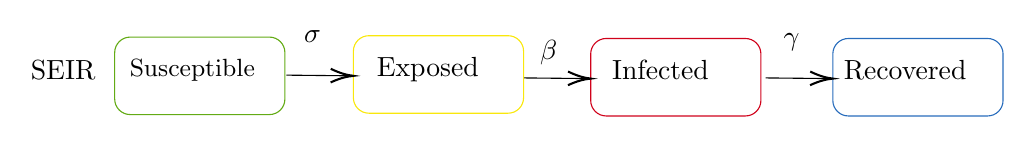
\begin{tikzpicture}[x=0.75pt,y=0.75pt,yscale=-1,xscale=1]
		%uncomment if require: \path (0,300); %set diagram left start at 0, and has
		%height of 300
		
		%Rounded Rect [id:dp9217887491174969] 
		\draw  [color={rgb, 255:red, 99; green, 171; blue, 21 }  ,draw opacity=1 ]
		(62.33,41.47) .. controls (62.33,37.34) and (65.68,34) .. (69.8,34) --
		(136.87,34) .. controls (140.99,34) and (144.33,37.34) .. (144.33,41.47) --
		(144.33,63.87) .. controls (144.33,67.99) and (140.99,71.33) .. (136.87,71.33)
		-- (69.8,71.33) .. controls (65.68,71.33) and (62.33,67.99) .. (62.33,63.87) --
		cycle ;
		%Rounded Rect [id:dp36097559929859013] 
		\draw  [color={rgb, 255:red, 208; green, 2; blue, 27 }  ,draw opacity=1 ]
		(291.67,42.13) .. controls (291.67,38.01) and (295.01,34.67) .. (299.13,34.67)
		-- (366.2,34.67) .. controls (370.32,34.67) and (373.67,38.01) .. (373.67,42.13)
		-- (373.67,64.53) .. controls (373.67,68.66) and (370.32,72) .. (366.2,72) --
		(299.13,72) .. controls (295.01,72) and (291.67,68.66) .. (291.67,64.53) --
		cycle ;
		%Straight Lines [id:da9742211892376831] 
		\draw    (259.33,53.67) -- (289.67,53.98) ; \draw [shift={(291.67,54)}, rotate =
			180.59] [color={rgb, 255:red, 0; green, 0; blue, 0 }  ][line width=0.75]
		(10.93,-3.29) .. controls (6.95,-1.4) and (3.31,-0.3) .. (0,0) .. controls
		(3.31,0.3) and (6.95,1.4) .. (10.93,3.29)   ;
		%Rounded Rect [id:dp37752716490425275] 
		\draw  [color={rgb, 255:red, 40; green, 108; blue, 188 }  ,draw opacity=1 ]
		(408.33,42.13) .. controls (408.33,38.01) and (411.68,34.67) .. (415.8,34.67) --
		(482.87,34.67) .. controls (486.99,34.67) and (490.33,38.01) .. (490.33,42.13)
		-- (490.33,64.53) .. controls (490.33,68.66) and (486.99,72) .. (482.87,72) --
		(415.8,72) .. controls (411.68,72) and (408.33,68.66) .. (408.33,64.53) -- cycle
		;
		%Straight Lines [id:da2512507786148114] 
		\draw    (376,53.67) -- (406.33,53.98) ; \draw [shift={(408.33,54)}, rotate =
			180.59] [color={rgb, 255:red, 0; green, 0; blue, 0 }  ][line width=0.75]
		(10.93,-3.29) .. controls (6.95,-1.4) and (3.31,-0.3) .. (0,0) .. controls
		(3.31,0.3) and (6.95,1.4) .. (10.93,3.29)   ;
		%Rounded Rect [id:dp4832950812851634] 
		\draw  [color={rgb, 255:red, 249; green, 231; blue, 9 }  ,draw opacity=0.99 ]
		(177.33,40.8) .. controls (177.33,36.68) and (180.68,33.33) .. (184.8,33.33) --
		(251.87,33.33) .. controls (255.99,33.33) and (259.33,36.68) .. (259.33,40.8) --
		(259.33,63.2) .. controls (259.33,67.32) and (255.99,70.67) .. (251.87,70.67) --
		(184.8,70.67) .. controls (180.68,70.67) and (177.33,67.32) .. (177.33,63.2) --
		cycle ;
		%Straight Lines [id:da02397316252168946] 
		\draw    (145,52.33) -- (175.33,52.65) ; \draw [shift={(177.33,52.67)}, rotate =
			180.59] [color={rgb, 255:red, 0; green, 0; blue, 0 }  ][line width=0.75]
		(10.93,-3.29) .. controls (6.95,-1.4) and (3.31,-0.3) .. (0,0) .. controls
		(3.31,0.3) and (6.95,1.4) .. (10.93,3.29)   ;
		
		
		% Text Node
		\draw (68.33,43.33) node [anchor=north west][inner sep=0.75pt]   [align=left]
		{{\small Susceptible}};
		% Text Node
		\draw (300.67,44) node [anchor=north west][inner sep=0.75pt]   [align=left]
		{Infected};
		% Text Node
		\draw (412.33,44) node [anchor=north west][inner sep=0.75pt]   [align=left]
		{Recovered};
		% Text Node
		\draw (266,34.07) node [anchor=north west][inner sep=0.75pt]    {$\beta $};
		% Text Node
		\draw (383.33,31.07) node [anchor=north west][inner sep=0.75pt]    {$\gamma $};
		% Text Node
		\draw (187.33,42.67) node [anchor=north west][inner sep=0.75pt]   [align=left]
		{Exposed};
		% Text Node
		\draw (152.33,29.73) node [anchor=north west][inner sep=0.75pt]    {$\sigma $};
		% Text Node
		\draw (20.67,44.33) node [anchor=north west][inner sep=0.75pt]   [align=left]
		{SEIR};
		
		
	\end{tikzpicture}
	
	} \caption{\textbf{Diagram of a dynamic compartmental model.}}
	\label{fig:dynamicmodel}
\end{figure}

The compartment flow is based on the order of the letters~\citep{amaku:2014}.
For example, an SEIR model states that individuals are initially susceptible to
the virus or disease, then they become exposed, infected, and finally recover.
The transition between states is not mandatory and depends on the model's
internal parameters, which aim to be as coherent as possible with reality. The
choice of a model depends primarily on the intrinsic characteristics of the
disease. The literature has proposed a set of different models considering
various types of compartments, such as \textbf{SEI}~\cite{Scoglio2021,
	Puntipa2023}, \textbf{SEIR}~\cite{Scoglio2021, Puntipa2023, Meng2023,
	da-silva:2020}, and \textbf{SIR}~\cite{Umar2022, Prasetyo2023, Srivastav2023},
among others.  Classical mathematical models are mainly based on compartmental
theory, and a system of \gls{ode} describes the changes between
states~\citep{da-silva:2020}.


% \chapter{Mathematical Models} \label{chapter:models}

Since routes may start and end at different nodes of $D$, we augment the digraph to $D' = (V', A')$  to include a dummy depot $0$ and a set of arcs such that $A' = \{(0, u), (u, 0)\}$, and $t_{u0} = t_{0u} = 0$, $\forall u \in V$. Consider $B(i)$ as the set of blocks touching node $i$, $V(b)$ as the set of vertices in block $b$, and the following sets of variables:

 \section{Model Without repeating Nodes}
 
\begin{itemize}
  \item $x_{ij}$: binary variable that indicates whether arc $(i, j) \in
    A'$ belongs to the route ($x_{ij} = 1$) or not ($x_{ij} = 0$);
  \item $y_{ib}$: binary variable that is valued 1 if node $i \in V$ is
    used as the starting point to service block $b \in B(i)$, and valued 0 otherwise; 
\end{itemize}

With these variables, the T-CBRP formulation reads:
\allowdisplaybreaks
\begin{align}
  \text{(T-CBRP) } & \max \sum_{i \in V} \sum_{b \in B} p_b y_{ib} & \label{eq:of}\\
  \nonumber \text{subject to:} & & \\
       & \sum_{a \in \delta^{-}(0)} x_{a} = \sum_{a' \in \delta^{+}(0)} x_{a'} = 1 & \label{eq:s-t-all} \\
       %
       & \sum_{a \in \delta^{-}(i)} x_{a} - \sum_{a' \in \delta^{+}(i)} x_{a'} = 0 & \ \forall i \in V \label{eq:flow-conservation} \\
       % & \sum_{i \in V'} \sum_{b \in B} f^I_b y_{ib} \leq I_{\max} & \label{eq:max-insecticide} \\
       %
       & \sum_{i \in V(b)} y_{ib} \leq 1 & \ \forall b \in B \label{eq:max-attend} \\
       %
       & \sum_{a \in \delta^{+}(i)} x_{a} \geq y_{ib} & \ \forall i \in V(b), b \in B \label{eq:in-path} \\
       %
       & \sum_{a \in A'} x_{a}t_{a} + \sum_{i \in V'} \sum_{b \in B} y_{ib}t_{b} \leq T & \label{eq:max-time} \\
       %
       & \sum_{a \in A(S)} x_{a} \leq |V(S)| - 1 & \ \forall S \subseteq V \label{eq:circuit-subtour-elimination} \\
       %
       & x \in \mathbb{B}^{|A'|} & \label{eq:dom-x} \\
       & y \in \mathbb{B}^{|V'| * |B|} & \label{eq:dom-y}
\end{align}

The T-CBRP formulation generates a tour that starts and ends at the dummy depot. The objective function~\eqref{eq:of} maximizes the profit collected from each block. Constraints~\eqref{eq:s-t-all}-\eqref{eq:flow-conservation} enforce flow conservation in each node. Constraints~\eqref{eq:max-attend} and~\eqref{eq:in-path} ensure that only one node is used as the starting point for servicing a block. Constraints~\eqref{eq:max-time} limit the time used by the route, considering different times whether the vehicle is servicing or not. Constraints~\eqref{eq:circuit-subtour-elimination} eliminate subcycles. Constraints~\eqref{eq:dom-x}-\eqref{eq:dom-y} define the domain of the variables.

The subcycle elimination constraints, exponentially large in the size of the input, 
can be replaced by the compact set of variables and constraints known as MTZ (Miller-Tucker-Zemlin). To this end, consider the following variables:

\begin{itemize}
    \item $w_{a}$: real variable representing the accumulated time in arc $a \in A'$.
\end{itemize}

Now it is possible to replace constraints \eqref{eq:circuit-subtour-elimination} with the following:

\begin{align}
  & w_{a'} \geq w_{a} + x_{a}t_{a} - (2 - x_{a'} - x_{a})T & \ \forall a \in \delta^{+}(i), a' \in \delta^{-}(i), i \in V' \label{eq:max-time-compact-leq} \\
   %
   & w_{a} \leq T & \ \forall a \in \delta^{+}(0) & \label{eq:max-time-compact}
\end{align}

Constraints~\eqref{eq:max-time-compact-leq} compute the accumulated time for each arc while  Constraints~\eqref{eq:max-time-compact} limit the amount of time used in the route. This new formulation has a number of constraints that grows polynomially with the size of the instance and the resulting route is equivalent to the formulation T-CBRP, i.e., a closed path.

\section{Models That Allows Repetitions os Arcs}

The first option is to use the above models with a new Graph create from the transitive closure of D.

The second options is to use the plannar input graph with the following model:

\begin{itemize}
  \item $x_{ij}$: integer variable that count how many times the arc $(i, j) \in A'$ was traveled in the route;
  \item $y_{b}$: binary variable that is valued 1 if block $b \in B(i)$ is serviced, and valued 0 otherwise; 
\end{itemize}

\begin{align}
  \text{(W-CBRP) } & \max \sum_{i \in V} \sum_{b \in B} p_b y_{b} & \label{eq:of}\\
  \nonumber \text{subject to:} & & \\
       & \sum_{a \in \delta^{-}(0)} x_{a} = \sum_{a' \in \delta^{+}(0)} x_{a'} = 1 & \label{eq:s-t-all} \\
       %
       & \sum_{a \in \delta^{-}(i)} x_{a} - \sum_{a' \in \delta^{+}(i)} x_{a'} = 0 & \ \forall i \in V \label{eq:flow-conservation} \\
       % & \sum_{i \in V'} \sum_{b \in B} f^I_b y_{ib} \leq I_{\max} & \label{eq:max-insecticide} \\
       %
       % & \sum_{i \in V(b)} y_{ib} \leq 1 & \ \forall b \in B \label{eq:max-attend} \\
       %
       & \sum_{a \in \delta^{+}(i)} x_{a} \geq y_{b} & \ \forall i \in V(b), b \in B \label{eq:in-path} \\
       %
       & \sum_{a \in A'} x_{a}t_{a} + \sum_{b \in B} y_{b}t_{b} \leq T & \label{eq:max-time} \\
       %
       & \sum_{a \in A(S)} x_{a} \leq |V(S)| - 1 + \sum_{a' \in \delta^{+}(S)} x_{a'} & \ \forall S \subseteq V \label{eq:new-walk-subtour-elimination} \\
       %
       & x \in \mathbb{Z}^{|A'|} & \label{eq:dom-x} \\
       & y \in \mathbb{B}^{|B|} & \label{eq:dom-y}
\end{align}


% \chapter{Heuristics}

\section{Constructive Heuristic}

How to connect blocks:

\begin{figure}[ht!]
  \centering
  \begin{subfigure}{0.49\textwidth}
      \centering
      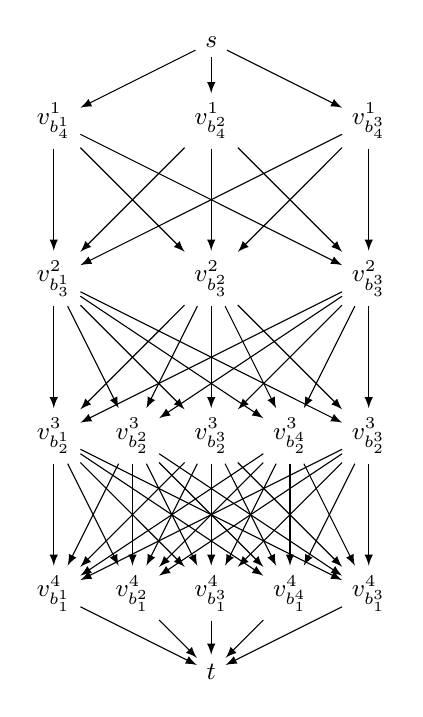
\begin{tikzpicture}[>=latex]
        \coordinate (s) at (2, 5);
        \coordinate (v11) at (0, 4);
        \coordinate (v12) at (2, 4);
        \coordinate (v13) at (4, 4);
        \coordinate (v21) at (0, 2);
        \coordinate (v22) at (2, 2);
        \coordinate (v23) at (4, 2);
        \coordinate (v31) at (0, 0);
        \coordinate (v32) at (1, 0);
        \coordinate (v33) at (2, 0);
        \coordinate (v34) at (3, 0);
        \coordinate (v35) at (4, 0);
        \coordinate (v41) at (0, -2);
        \coordinate (v42) at (1, -2);
        \coordinate (v43) at (2, -2);
        \coordinate (v44) at (3, -2);
        \coordinate (v45) at (4, -2);
        \coordinate (t)   at (2, -3);
        \node (ns)   at (s)   {\small$s$};
        \node (nv11) at (v11) {\small$v^1_{b_4^1}$};
        \node (nv12)  at (v12) {\small$v^1_{b_4^2}$};
        \node (nv13)  at (v13) {\small$v^1_{b_4^3}$};
        \node (nv21)  at (v21) {\small$v^2_{b_3^1}$};
        \node (nv22)  at (v22) {\small$v^2_{b_3^2}$};
        \node (nv23)  at (v23) {\small$v^2_{b_3^3}$};
        \node (nv31)  at (v31) {\small$v^3_{b_2^1}$};
        \node (nv32)  at (v32) {\small$v^3_{b_2^2}$};
        \node (nv33)  at (v33) {\small$v^3_{b_2^3}$};
        \node (nv34)  at (v34) {\small$v^3_{b_2^4}$};
        \node (nv35)  at (v35) {\small$v^3_{b_2^3}$};
        \node (nv41)  at (v41) {\small$v^4_{b_1^1}$};
        \node (nv42)  at (v42) {\small$v^4_{b_1^2}$};
        \node (nv43)  at (v43) {\small$v^4_{b_1^3}$};
        \node (nv44)  at (v44) {\small$v^4_{b_1^4}$};
        \node (nv45)  at (v45) {\small$v^4_{b_1^3}$};
        \node (nt)    at (t)   {\small$t$};
        % arcs
        \def\arcs{%
          ns nv11
          ns nv12
          ns nv13
          nv11 nv21
          nv11 nv22
          nv11 nv23
          nv12 nv21
          nv12 nv22
          nv12 nv23
          nv13 nv21
          nv13 nv22
          nv13 nv23
          nv21 nv31
          nv21 nv32
          nv21 nv33
          nv21 nv34
          nv21 nv35
          nv22 nv31
          nv22 nv32
          nv22 nv33
          nv22 nv34
          nv22 nv35
          nv23 nv31
          nv23 nv32
          nv23 nv33
          nv23 nv34
          nv23 nv35
          nv31 nv41
          nv31 nv42
          nv31 nv43
          nv31 nv44
          nv31 nv45
          nv32 nv41
          nv32 nv42
          nv32 nv43
          nv32 nv44
          nv32 nv45
          nv33 nv41
          nv33 nv42
          nv33 nv43
          nv33 nv44
          nv33 nv45
          nv34 nv41
          nv34 nv42
          nv34 nv43
          nv34 nv44
          nv34 nv45
          nv35 nv41
          nv35 nv42
          nv35 nv43
          nv35 nv44
          nv35 nv45
          nv41 nt
          nv42 nt
          nv43 nt
          nv44 nt
          nv45 nt
        }
        \readarray\arcs\Arcs[9,2]
        % print arcs
        \drawArcs{\Arcs}{\ArcsROWS}{->}
      \end{tikzpicture}
      \caption{$D^G$ example.}
  \end{subfigure}
  \begin{subfigure}{0.49\textwidth}
      \centering
      \begin{tikzpicture}[>=latex]
        \coordinate (s) at (2, 5);
        \coordinate (v11) at (0, 4);
        \coordinate (v12) at (2, 4);
        \coordinate (v13) at (4, 4);
        \coordinate (v21) at (0, 2);
        \coordinate (v22) at (2, 2);
        \coordinate (v23) at (4, 2);
        \coordinate (v31) at (0, 0);
        \coordinate (v32) at (1, 0);
        \coordinate (v33) at (2, 0);
        \coordinate (v34) at (3, 0);
        \coordinate (v35) at (4, 0);
        \coordinate (v41) at (0, -2);
        \coordinate (v42) at (1, -2);
        \coordinate (v43) at (2, -2);
        \coordinate (v44) at (3, -2);
        \coordinate (v45) at (4, -2);
        \coordinate (t)   at (2, -3);
        \node (ns)   at (s)   {\small$s$};
        \node (nv11) at (v11) {\small$v^1_{b_4^1}$};
        \node (nv12)  at (v12) {\small$v^1_{b_4^2}$};
        \node (nv13)  at (v13) {\small$v^1_{b_4^3}$};
        \node (nv21)  at (v21) {\small$v^2_{b_3^1}$};
        \node (nv22)  at (v22) {\small$v^2_{b_3^2}$};
        \node (nv23)  at (v23) {\small$v^2_{b_3^3}$};
        \node (nv31)  at (v31) {\small$v^3_{b_2^1}$};
        \node (nv32)  at (v32) {\small$v^3_{b_2^2}$};
        \node (nv33)  at (v33) {\small$v^3_{b_2^3}$};
        \node (nv34)  at (v34) {\small$v^3_{b_2^4}$};
        \node (nv35)  at (v35) {\small$v^3_{b_2^3}$};
        \node (nv41)  at (v41) {\small$v^4_{b_1^1}$};
        \node (nv42)  at (v42) {\small$v^4_{b_1^2}$};
        \node (nv43)  at (v43) {\small$v^4_{b_1^3}$};
        \node (nv44)  at (v44) {\small$v^4_{b_1^4}$};
        \node (nv45)  at (v45) {\small$v^4_{b_1^3}$};
        \node (nt)    at (t)   {\small$t$};
        % arcs
        \def\arcs{%
          nv11 nv23
          nv23 nv32
        }
        \readarray\arcs\Arcs[9,2]
        % print arcs
        \drawArcs{\Arcs}{\ArcsROWS}{->}
      \end{tikzpicture}
      \caption{Obtained tour with $k = 3$.}
  \end{subfigure}
  \caption{Block connection heuristic.}
  \label{fig:brkga_example}
\end{figure}

% \begin{algorithm}[!ht]
% \scriptsize
% % \DontPrintSemicolon 
% 	\caption{\label{alg:stochastic-construction} Stochastic Initial Solution}
% 	\KwIn{Graph G, Scenarios S, Time T}
% 	\KwOut{$X, Y$ set of |S| routes and their respective attended blocks}

%     $P_0 \leftarrow$ update profits from first stage\;
%     $T_{UB} = 1.0 * T$\;
%     $T_{LB} = 0.5 * T$\;
    
% 	\Repeat{close the gap between $T_{UB}$ and $T_{LB}$}{ \label{line:rep-beg} 
%         $T' \leftarrow $ reserved time to attend (from binary search)\; 
%         $Y_0, X_0 \leftarrow$ solve first stage route ($P_0, T'$)\;

%         \For{$s = 1, 2, \dots, |S|$}{
%             $P_s \leftarrow$ update second stage profit $(Y_0)$\;
%             $Y_s, X_s \leftarrow$ solve second stage route ($P_s, T'$)\;
%             $C_k(x) \leftarrow 0$\; 
%             \For{$j = 1, 2, \dots, n$}{
%                 \uIf{$k \neq j$}{
%                    $C_k(x) \leftarrow C_k(x) + (c_{kj} * x_j)$\;
%                 }
%             } \label{line:calc-ckx-end}
            
%            \uIf{$C_k(x) < C_k/2$ \textbf{and} $x_k = 0$}{\label{line:if-change}
%                 $x_k \leftarrow 1$\;
%             } 
%             \uElseIf {$C_k(x) > C_k/2$ \textbf{and} $x_k = 1$} {
%               $x_k \leftarrow 0$\;
%             } \label{line:if-change-two}
%         }
% 	} \label{line:rep-end}
% 	\Return{$x$}\;

% \end{algorithm}

% O corpo da dissertação ou tese começa aqui:
% \chapter{Introdução}

% Lorem ipsum dolor sit amet, consectetur adipiscing elit, sed do eiusmod
% tempor incididunt ut labore et dolore magna aliqua. Ut enim ad minim
% veniam, quis nostrud exercitation ullamco laboris nisi ut aliquip ex ea
% commodo consequat. Duis aute irure dolor in reprehenderit in voluptate
% velit esse cillum dolore eu fugiat nulla pariatur. Excepteur sint occaecat
% cupidatat non proident, sunt in culpa qui officia deserunt mollit anim id
% est laborum.

% \begin{table}
% \caption[Shorter table caption]{Table caption caption caption caption
%   caption caption caption caption caption caption caption caption caption
%   caption caption caption caption caption caption caption caption caption
%   caption caption.}
% \label{t:label0}
% \begin{center}
% \begin{tabular}{|c|c|}
% \hline
% a & b \\\hline
% c & d \\\hline
% \end{tabular}
% \end{center}
% \end{table}

% Lorem ipsum dolor sit amet, consectetur adipiscing elit, sed do eiusmod
% tempor incididunt ut labore et dolore magna aliqua. Ut enim ad minim
% veniam, quis nostrud exercitation ullamco laboris nisi ut aliquip ex ea
% commodo consequat. Duis aute irure dolor in reprehenderit in voluptate
% velit esse cillum dolore eu fugiat nulla pariatur. Excepteur sint occaecat
% cupidatat non proident, sunt in culpa qui officia deserunt mollit anim id
% est laborum.

% Lorem ipsum dolor sit amet, consectetur adipiscing elit, sed do eiusmod
% tempor incididunt ut labore et dolore magna aliqua. Ut enim ad minim
% veniam, quis nostrud exercitation ullamco laboris nisi ut aliquip ex ea
% commodo consequat. Duis aute irure dolor in reprehenderit in voluptate
% velit esse cillum dolore eu fugiat nulla pariatur. Excepteur sint occaecat
% cupidatat non proident, sunt in culpa qui officia deserunt mollit anim id
% est laborum.

% Lorem ipsum dolor sit amet, consectetur adipiscing elit, sed do eiusmod
% tempor incididunt ut labore et dolore magna aliqua. Ut enim ad minim
% veniam, quis nostrud exercitation ullamco laboris nisi ut aliquip ex ea
% commodo consequat. Duis aute irure dolor in reprehenderit in voluptate
% velit esse cillum dolore eu fugiat nulla pariatur. Excepteur sint occaecat
% cupidatat non proident, sunt in culpa qui officia deserunt mollit anim id
% est laborum.

% Lorem ipsum dolor sit amet, consectetur adipiscing elit, sed do eiusmod
% tempor incididunt ut labore et dolore magna aliqua. Ut enim ad minim
% veniam, quis nostrud exercitation ullamco laboris nisi ut aliquip ex ea
% commodo consequat. Duis aute irure dolor in reprehenderit in voluptate
% velit esse cillum dolore eu fugiat nulla pariatur. Excepteur sint occaecat
% cupidatat non proident, sunt in culpa qui officia deserunt mollit anim id
% est laborum~\cite{2014-bic,2015-ela}.

% \begin{figure}
% \centerline{\includegraphics[scale=0.2]{logo-ic-unicamp.eps}}
% \caption[Shorter figure caption]{Figure Caption caption caption caption
%   caption caption caption caption caption caption caption caption caption
%   caption caption caption caption caption caption caption caption caption
%   caption caption.}
% \label{f:label1}
% \end{figure}

% Lorem ipsum dolor sit amet, consectetur adipiscing elit, sed do eiusmod
% tempor incididunt ut labore et dolore magna aliqua. Ut enim ad minim
% veniam, quis nostrud exercitation ullamco laboris nisi ut aliquip ex ea
% commodo consequat\footnote{Footnote footnote footnote footnote footnote
%   footnote footnote footnote footnote footnote footnote footnote footnote
%   footnote footnote footnote.}.  Duis aute irure dolor in reprehenderit in
% voluptate velit esse cillum dolore eu fugiat nulla pariatur. Excepteur sint
% occaecat cupidatat non proident, sunt in culpa qui officia deserunt mollit
% anim id est laborum.


% \chapter{Hipóteses}


% \chapter{Resultados}


% \chapter{Conclusões}



% As referências:
\bibliographystyle{plain}
\bibliography{ic-tese-v3}


% Os anexos, se houver, vêm depois das referências:
% \appendix
% \chapter{Anexo 1}
% \chapter{Anexo 2}

\end{document}
